%!TEX root = ./template-skripsi.tex
%-------------------------------------------------------------------------------
%                            	BAB IV
%               		KESIMPULAN DAN SARAN
%-------------------------------------------------------------------------------

\chapter{HASIL DAN PEMBAHASAN}

\section{Pembahasan}

Aplikasi pendukung teknologi perikanan modern, dirancang dengan menggunakan metode Scrum. Pada metode Scrum, proses pengembangan sistem dilakukan secara bertahap yang disebut dengan Sprint. Pada penelitian ini terdapat sembilan Sprint dimana satu putaran Sprint memiliki durasi selama dua minggu. Pada tiap awal pekan, dilakukan perencanaan Sprint Backlog berdasarkan Product Backlog telah disepakati. Adapun laporan setiap Sprint yang dilakukan pada proses pengembangan sistem adalah sebagai berikut:

%!TEX root = ./template-skripsi.tex

\subsection{\textit{Sprint 1}}

	\textit{Sprint-1} dilakukan sepekan pada tanggal 23 Agustus 2022 sampai dengan 30 Agustus 2022. \textit{Story} pertama pada \textit{product backlog} yaitu membuat halamn dashboard dipecah menjadi beberapa \textit{task} sebagai berikut.


 \begin{longtable}[c]{@{} |p{1cm}|p{4cm}|p{5cm}|p{3cm}| @{}}
 \caption{\textit{Sprint 1} \label{sprint1_table}}\\


 \hline
  \multirow{1}{=}{\centering{\textbf{No}}} & \multirow{1}{=}{\centering{\textbf{\textit{Story}}}} & \multirow{1}{=}{\centering{\textbf{\textit{Task}}}} & \multirow{1}{=}{\centering{\textbf{\textit{Status}}}}\\
 \endfirsthead

 \hline
  \multirow{1}{=}{\centering{\textbf{No}}} & \multirow{1}{=}{\centering{\textbf{\textit{Story}}}} & \multirow{1}{=}{\centering{\textbf{\textit{Task}}}} & \multirow{1}{=}{\centering{\textbf{\textit{Status}}}}\\
 \endhead

 \hline
 \endfoot

 \hline
 \endlastfoot

 \hline
 1 & Membuat Halaman Dashboard &  Membuat \textit{Mock-up UI} halaman dashboard  &  selesai \\
 \hline
 2 & & Menerapkan struktur direktori dan membuat class diagram & selesai\\
 \hline
 3 & & Menerapkan \textit{Mock-up UI} halaman dashboard ke Flutter & selesai\\
 \hline
 4 & & Mengintegrasikan halaman home ke \textit{webservice} & selesai\\
 \hline
 \end{longtable}

Pada sprint pertama ini story yang di pilih untuk di uraikan pada sprint kali ini adalah membuat halaman dashboard. Tujuan dari \textit{sprint-1} ini adalah membuat halaman home dan mengintegrasikan halaman tersebut dengan webservice yang sudah dibuat oleh penelitian Andri Rahmanto. Kendala yang dialami penilis pada sprint kali ini adalah diperlukannya waktu traning terhadap bahasa pemrograman dan framework yang digunakan dalam melakukan pengembangan aplikasi,  penulis menggunakan \textit{GitHub Projects} seperti pada gambar \ref{gambar:sprint1_projects}.
	
\begin{figure}[H]
	\centering
	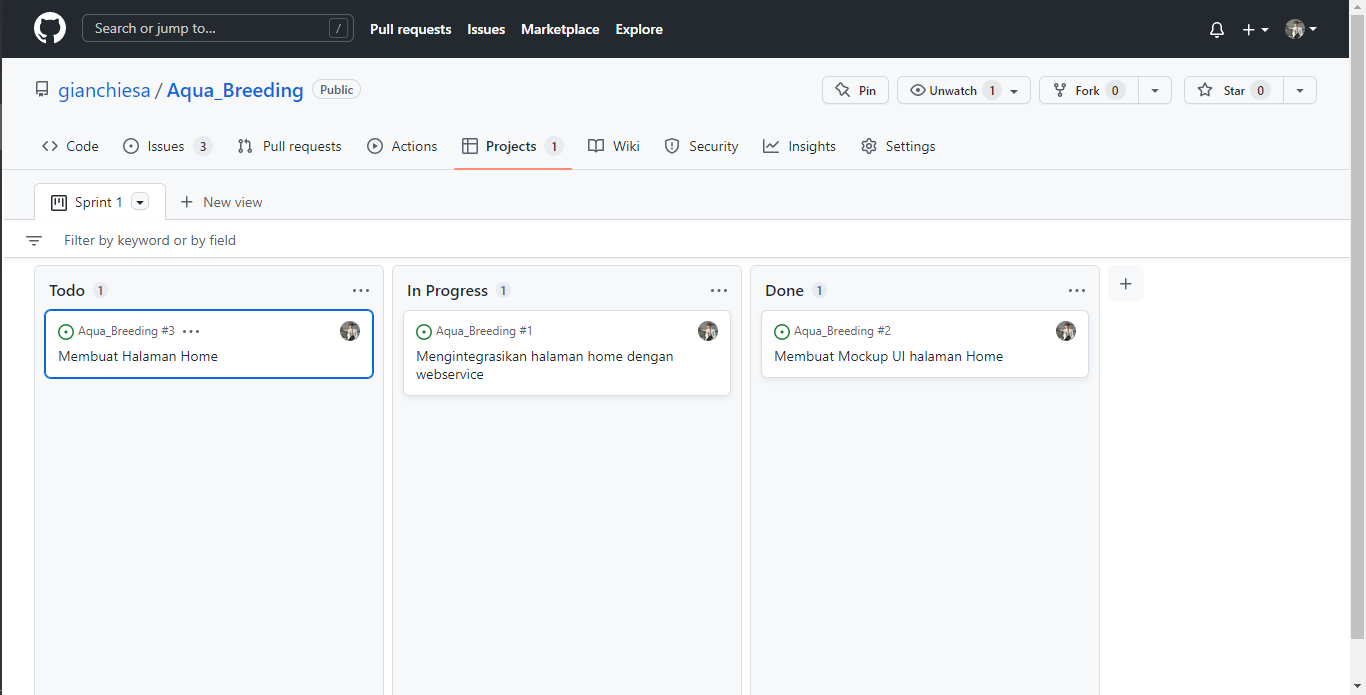
\includegraphics[keepaspectratio, width=14cm]{gambar/githubprojectgian}
	\caption{\textit{Github Projects Sprint-1}}
	\label{gambar:sprint1_projects}
\end{figure}
	
Terdapat 3 kolom pada \textit{project} yang dibuat, yaitu \textit{to do}, \textit{in progress}, dan \textit{completed}. Setiap \textit{task} yang perlu dikerjakan akan ditulis dan dimasukkan ke dalam kolom \textit{to do}, selanjutnya \textit{task} yang sedang dikerjakan akan dipindahkan ke kolom \textit{in progress}, dan jika task sudah selesai akan dipindahkan ke kolom \textit{completed}. Berikut merupakan hasil dari pengerjaan yang dilakukan selama \textit{sprint 1}.

\begin{enumerate}[listparindent=2em]
	
	\item{\textit{Membuat Mock-up UI Halaman Dashboard}}
	
	Pembuatan konten dan fitur yang terdapat pada \textit{mock-up UI} halaman home dilakukan berdasarkan persetujuan product owner dan scrum master pada meeting sebelumnya. Mock-up UI dibuat menggunakan platform figma.
	
	\begin{figure}[H]
	\centering
	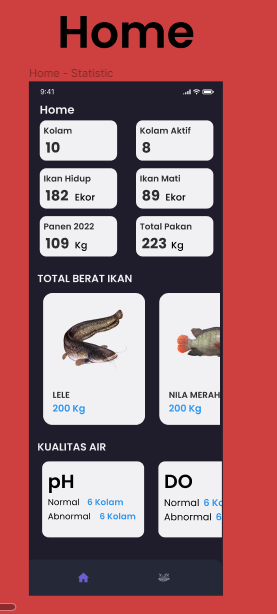
\includegraphics[keepaspectratio, width=4cm]{gambar/mockuphome}
	\caption{\textit{Mock-up UI Halaman Dashboard}}
	\label{gambar:mockuphome}
	\end{figure}

	Lalu selanjutnya dibuat prototype agar product owner dan scrum master dapat lebih mengerti bagaimana konten dan fitur tersebut berjalan saat akan dikembangkan seperti pada gambar \ref{gambar:protohome}.

	\begin{figure}[H]
	\centering
	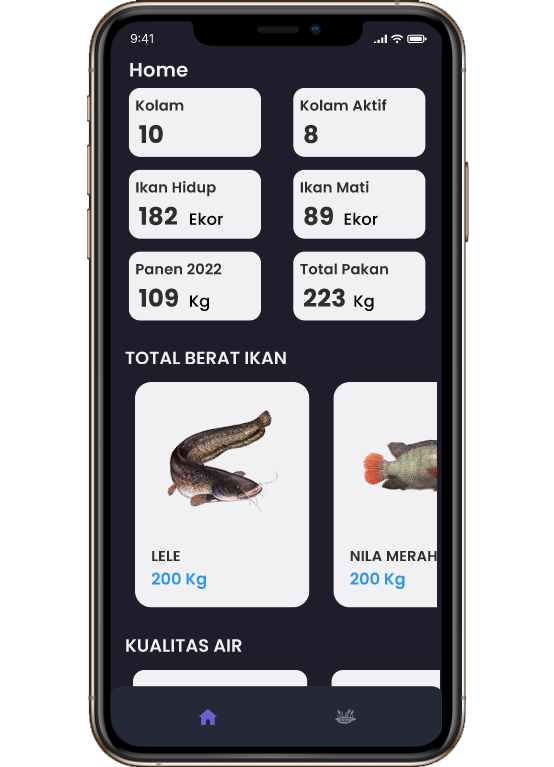
\includegraphics[keepaspectratio, width=5cm]{gambar/protohome}
	\caption{\textit{Prototype Halaman Dashboard}}
	\label{gambar:protohome}
	\end{figure}
	
	\item{\textit{Menetapkan Struktor Direktori}}

	Sebelum menerapkan Mockup-UI kedalam code, penulis membuat atau menetapkan struktur direktori file agar memudahkan penulis untuk melakukan proses pengembangan untuk kedepannya. Terdapat 4 direktori yang penulis buat pada penelitian kal ini, yaitu models, controllers, pages, dan services. Direktori models akan memuat file yang berfungsi sebagai model class, lalu pada direktori contoller berisi file controller-controller yang akan digunakan pada suatu halaman/fitur untuk memanipulasi/mengolah data yang didapat dari services. Direktori services berisi file yang digunakan untuk berinteraksi dengan dunia luar seperti pemanggilan API dan membuat network request, untuk direktori pages memuat file UI halaman.

	\begin{figure}[H]
	\centering
	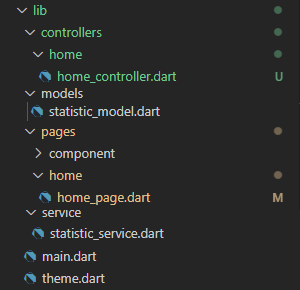
\includegraphics[keepaspectratio, width=7cm]{gambar/homedirektori}
	\caption{\textit{Struktur Direktori}}
	\label{gambar:homedirektori}
	\end{figure}

	\item{\textit{Class Diagram}}
	
	Class Diagram menggambarkan kelas-kelas yang akan dipakai oleh sistem. Umumnya terdapat 3 kelas pada setiap module yaitu class model, controller, dan view. Pada sprint-1 penelitian kali ini penulis membuat 4 class yaitu model, view , controller, dan service.
	 
	\begin{figure}[H]
	\centering
	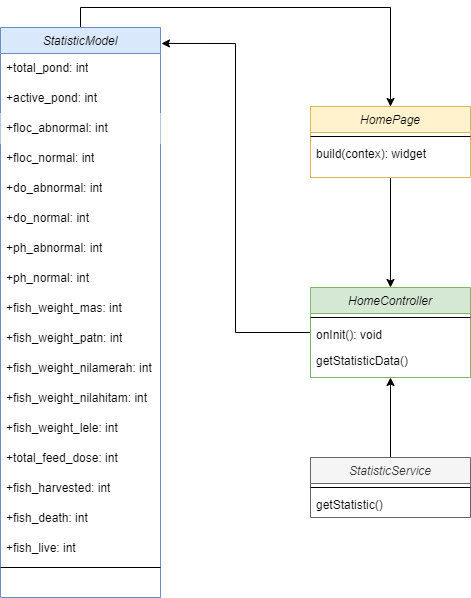
\includegraphics[keepaspectratio, width=6cm]{gambar/CDfishnew}
	\caption{\textit{Class Diagram Sprint-1}}
	\label{gambar:classdiagram}
	\end{figure}

	Pada gambar \ref{gambar:classdiagram} class HomePage sebagai view menginisiasi controller dari interaksi dengan user, lalu controller akan memanggil mengfetch data dari service class dan memasukan data tersebut ke model class, setelah itu model class akan memberi tahu sistem jika data sudah terupdate dan akan mengirimkan data tersebut kembali ke view.

	\item{\textit{Menerapkan Mockup-UI Halaman Dashboard kedalam code flutter}}
	
	Setelah \textit{mock-up UI Halaman Dashboard} hingga prototype dibuat, akan dilakukan pengimplementasian \textit{mock- up UI} ke dalam aplikasi menggukan flutter. Pada lampiran 2 terdapat source code dari implementasi halaman home yang dikelompokan berdasarkan section.

	\item{\textit{Mengitegrasikan Halaman Dashboard dengan webservice}}
	
	Sebelumnya, setiap data pada halaman home masih berupa data dummy sehingga perlu diintegrasikan dengan webservice agar aplikasi dapat berjalan dengan data yang asli. pada lampiran 6 terdapat langkah-langkah untuk mengintegrasikan halaman dashboard dengan webservice.
	

\item{Sprint 1 Review dan Sprint 2 Planning}

Sprint 1 diakhiri dengan melakukan weekly meeting pada hari selasa dengan agenda melakukan review dan testing terkait hasil sprint 1 dan melakukan planning untuk sprint 2 dengan rincian:
\begin{enumerate}
	\item{\textit{Review dan Testing hasil dari sprint 1}}

	Telah dilakukan review dan testing oleh penulis selaku developer dengan Scrum Master. Setelah dilakukan testing, Scrum Master menyimpulkan bahwa fitur pada halaman dashboard telah berjalan dengan baik.

	\begin{longtable}{| p{8cm} | c | c | l |}
		\caption{Unit testing Halaman Dashboard.\label{table:unit_testing_fitur_dashboard}}\\
		\hline
		\multirow{2}{*}{Skenario Pengujian} & \multicolumn{2}{l|}{Kesesuaian} & \multirow{2}{*}{Kesimpulan} \\ 
		\cline{2-3}
		  & \multicolumn{1}{l|}{sesuai} & tidak sesuai & \\ 
		\hline
		\hline
		\endfirsthead
		\hline
		\multirow{2}{*}{Skenario Pengujian} & \multicolumn{2}{l|}{Kesesuaian} & \multirow{2}{*}{Kesimpulan} \\ 
		\cline{2-3}
		  & \multicolumn{1}{l|}{sesuai} & tidak sesuai &  \\ 
		\hline
		\hline
		\endhead
		\hline
		\endfoot
		
		
		\hline\hline
		\endlastfoot
		 Ketika mengisi form login dengan data yang sesuai kemudian menekan submit, maka akan masuk ke halaman dashboard & \Checkmark &  & Diterima \\ 
		\hline
		 Saat tombol kolam ditekan maka akan muncul halaman yang menampilkan list kolam & \Checkmark & & Diterima \\ 
		\hline
		\end{longtable}

	\begin{figure}[H]
	\centering
	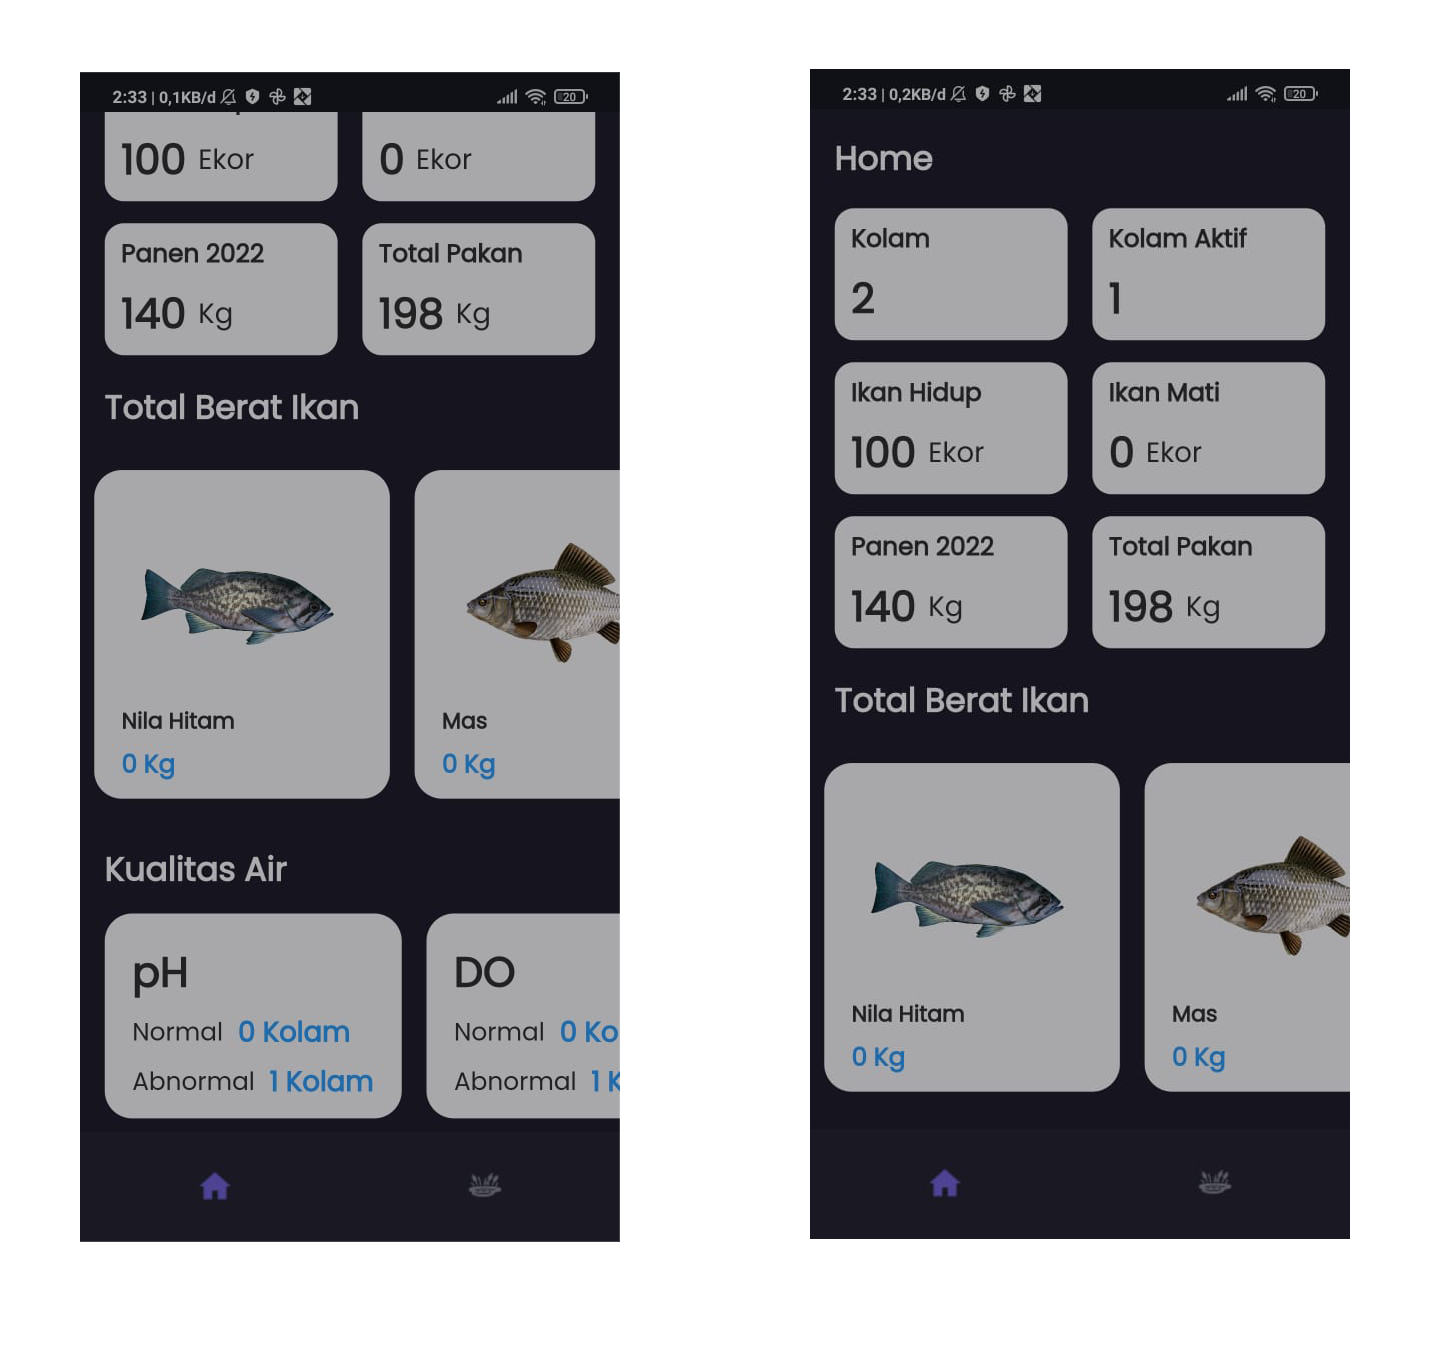
\includegraphics[keepaspectratio, width=7cm]{gambar/ssaqua}
	\caption{\textit{Screenshot dari Halaman Home yang telah selesai}}
	\label{gambar:mockuphome}
	\end{figure}

	\item{\textit{Sprint Planning untuk Sprint 2}}
	
	Planning untuk sprint 2 yakni membuat fitur registrasi kolam dan aktifasi musim budidaya pada aplikasi \textit{Assistive Aquaculture Breeding Management}.
\end{enumerate}
\end{enumerate}
`	
%!TEX root = ./template-skripsi.tex
\subsection{\textit{Sprint 2}}

	\textit{Sprint-2} dilakukan sepekan pada tanggal 30 Agustus 2022 sampai dengan 6 September 2022. \textit{Story} kedua pada \textit{product backlog} yaitu membuat fitur registrasi kolam dan aktivasi musim budidaya dipecah menjadi beberapa \textit{task} sebagai berikut.


 \begin{longtable}[c]{@{} |p{1cm}|p{4cm}|p{5cm}|p{3cm}| @{}}
 \caption{\textit{Sprint 2} \label{sprint2_table}}\\


 \hline
  \multirow{1}{=}{\centering{\textbf{No}}} & \multirow{1}{=}{\centering{\textbf{\textit{Story}}}} & \multirow{1}{=}{\centering{\textbf{\textit{Task}}}} & \multirow{1}{=}{\centering{\textbf{\textit{Status}}}}\\
 \endfirsthead

 \hline
  \multirow{1}{=}{\centering{\textbf{No}}} & \multirow{1}{=}{\centering{\textbf{\textit{Story}}}} & \multirow{1}{=}{\centering{\textbf{\textit{Task}}}} & \multirow{1}{=}{\centering{\textbf{\textit{Status}}}}\\
 \endhead

 \hline
 \endfoot

 \hline
 \endlastfoot

 \hline
 1 & Membuat fitur registrasi kolam dan aktivasi musim budidaya &  Membuat \textit{Mock-up UI} halaman list kolam, registrasi kolam, detail kolam, aktivasi dan deaktivasi kolam &  selesai \\
 \hline
 2 & & Menerapkan struktur direktori dan membuat class diagram & selesai\\
 \hline
 3 & & Menerapkan \textit{Mock-up UI}  halaman list kolam, registrasi kolam, detail kolam, aktivasi dan deaktivasi kolam & selesai\\
 \hline
 4 & & Mengintegrasikan halaman list kolam, registrasi kolam, detail kolam, aktivasi dan deaktivasi kolam ke \textit{webservice} & next sprint\\
 \hline
 \end{longtable}

Pada sprint ini story yang di pilih untuk di uraikan pada sprint kali ini adalah membuat fitur registrasi kolam dan aktivasi musim budidaya . Tujuan dari \textit{sprint-2} ini adalah membuat halaman list kolam, registrasi kolam, detail kolam, aktivasi dan deaktivasi kolam dan mengintegrasikan halaman tersebut dengan webservice. Kendala yang dialami penilis pada sprint kali ini adalah banyaknya fitur yang harus di aplikasikan sehingga ada task yang harus dilanjukan pada sprint berikutnya. Berikut merupakan hasil dari pengerjaan yang dilakukan selama \textit{sprint 2}.

\begin{enumerate}[listparindent=2em]
	
	\item{\textit{Membuat Mock-up UI Halaman List kolam, Registrasi kolam, Detail kolam, Aktivasi dan Deaktivasi kolam}}
	
	Pembuatan konten dan fitur yang terdapat pada \textit{mock-up UI} halaman list kolam, registrasi kolam, detail kolam, aktivasi dan deaktivasi kolam dilakukan berdasarkan persetujuan product owner dan scrum master pada meeting sebelumnya. Mock-up UI dibuat menggunakan platform figma.
	
	\begin{figure}[H]
	\centering
	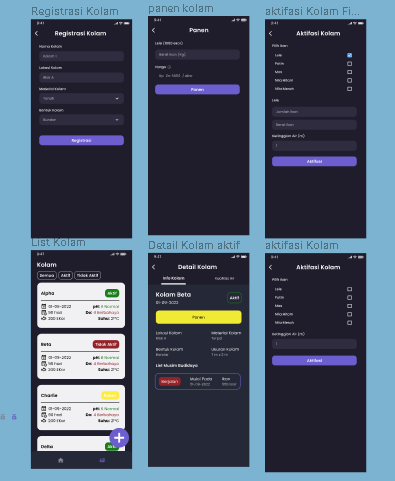
\includegraphics[keepaspectratio, width=4cm]{gambar/mockupsprint2}
	\caption{\textit{Mock-up UI List kolam, Registrasi kolam, Detail kolam, Aktivasi dan Deaktivasi kolam}}
	\label{gambar:mockupsprint2}
	\end{figure}

	\item{\textit{Class Diagram}}
	
	Class Diagram menggambarkan kelas-kelas yang akan dipakai oleh sistem. Umumnya terdapat 3 kelas pada setiap module yaitu class model, controller, dan view. Pada sprint-2 penelitian kali ini penulis membuat 4 class yaitu model yang berwarna biru, view berwarna oranye, controller yang berwarna hijau, dan service yang berwarna kuning.
	 
	 \begin{figure}[H]
	 \centering
	 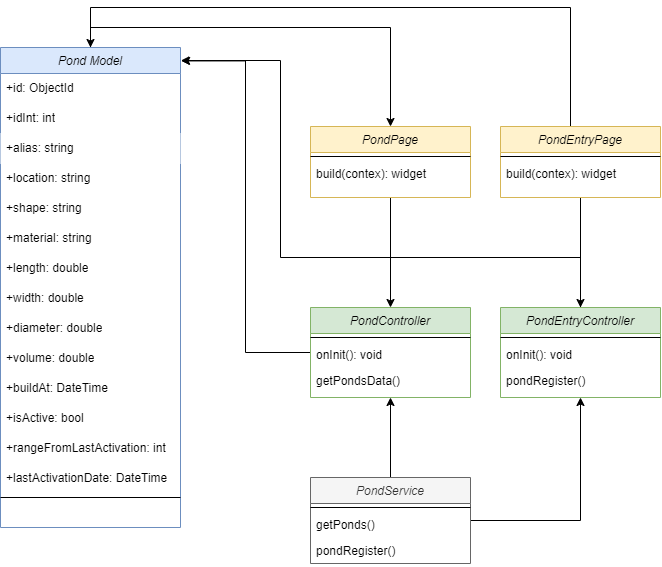
\includegraphics[keepaspectratio, width=6cm]{gambar/pondcd}
	 \caption{\textit{Class Diagram Fitur Koam Sprint-2}}
	 \label{gambar:pondcd}
	 \end{figure}

	 \begin{figure}[H]
	 \centering
	 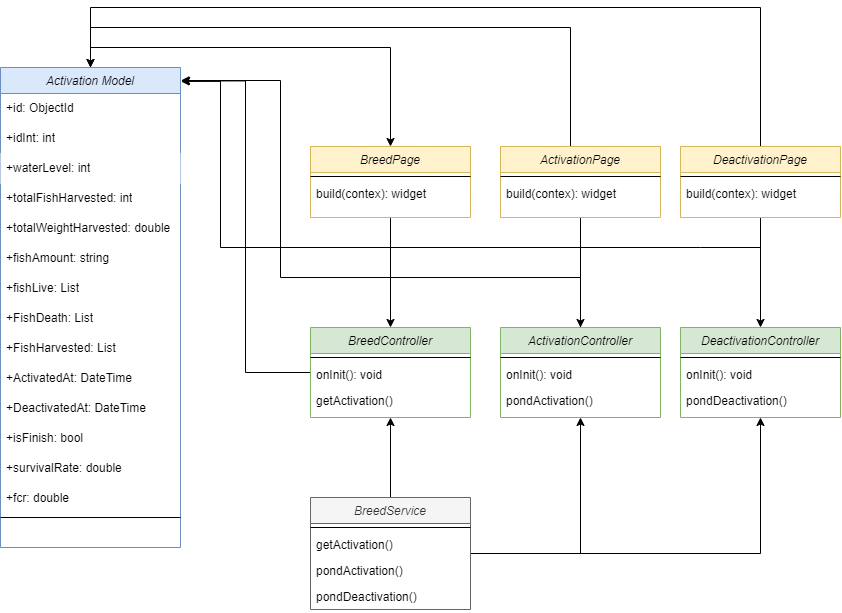
\includegraphics[keepaspectratio, width=6cm]{gambar/activationcd}
	 \caption{\textit{Class Diagram Fitur Aktivasi dan Deaktivasi Sprint-2}}
	 \label{gambar:activationcd}
	 \end{figure}

	\item{\textit{Menerapkan mockup-UI  halaman list kolam, registrasi kolam, detail kolam, aktivasi dan deaktivasi kedalam code flutter}}
	
	Setelah \textit{mock-up UI  halaman list kolam, registrasi kolam, detail kolam, aktivasi dan deaktivasi} dibuat, akan dilakukan pengimplementasian \textit{mock- up UI} ke dalam aplikasi menggukan flutter. Berikut adalah source code dari implementasi halaman list kolam, registrasi kolam, detail kolam, aktivasi dan deaktivasi yang terdapat pada lampiran 3 dan menghasilkan output halaman sebagai berikut

	\begin{figure}[H]
	\centering
	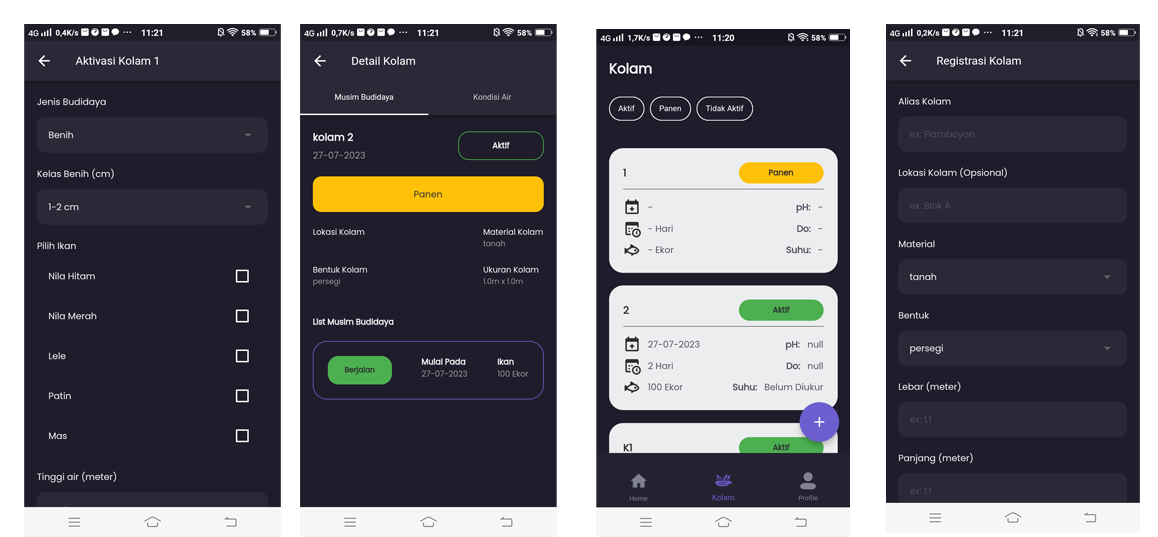
\includegraphics[keepaspectratio, width=8cm]{gambar/sssprint2}
	\caption{\textit{Output dari code pada sprint 2}}
	\label{gambar:sssprint4}
	\end{figure}

\item{Analisis \textit{User Experience}} 
 
pada halaman halaman list kolam terdapat card yang berisi informasi yang berguna bagi para pembudidaya untuk melakukan pemantauan terkait aktivitas yang terdapat pada masing-masing kolam. Sementara pada halaman registrasi kolam, pembudidaya harus memasukan data yang diperlukan untuk menambahkan kolam sesuai dengan kesepakatan saat meeting. Lalu pada halaman detail kolam terdapat data kolam terkait dan list musim budidaya yang telah berjalan di kolam tersebut. Sama halnya dengan aktivasi dan deaktivasi pembudidaya harus memasukan data yang diperlukan sesuai dengan kesepakatan saat meeting.


\item{Sprint 2 Review dan Sprint 3 Planning}

Sprint 2 diakhiri dengan melakukan weekly meeting pada hari selasa dengan agenda melakukan review dan testing terkait hasil sprint 2 dan melakukan planning untuk sprint 3 dengan rincian:
\begin{enumerate}
	\item{\textit{Review dan Testing hasil dari sprint 2}}

	Telah dilakukan review dan testing oleh penulis selaku developer dengan Scrum Master. Setelah dilakukan testing, Scrum Master menyimpulkan bahwa penerapan fitur pada halaman list kolam, detail kolam, aktivasi kolam, deaktivasi kolam telah berjalan dengan baik namun belum di integrasikan dengan data dari API sehingga akan dilanjutkan kedalam sprint berikutnya.

	\item{\textit{Sprint Planning untuk Sprint 3}}
	
	Planning untuk sprint 3 yakni membuat fitur pemberian pakan pada aplikasi \textit{Assistive Aquaculture Breeding Management}.
\end{enumerate}
\end{enumerate}
%!TEX root = ./template-skripsi.tex
\subsection{\textit{Sprint 3}}

	\textit{Sprint-3} dilakukan sepekan pada tanggal 6 September 2022 sampai dengan 13 September 2022. \textit{Story} ketiga  pada \textit{product backlog} yaitu membuat fitur pemberian pakan, ditambah dengan melanjutkan bagian yang belum selesai dari sprint sebelumnya yaitu mengintegrasikan halaman list kolam, registrasi kolam, aktivasi kolam, dan deaktivasi kolam dipecah menjadi beberapa \textit{task} sebagai berikut.


 \begin{longtable}[c]{@{} |p{1cm}|p{4cm}|p{5cm}|p{3cm}| @{}}
 \caption{\textit{Sprint 3} \label{sprint3_table}}\\


 \hline
  \multirow{1}{=}{\centering{\textbf{No}}} & \multirow{1}{=}{\centering{\textbf{\textit{Story}}}} & \multirow{1}{=}{\centering{\textbf{\textit{Task}}}} & \multirow{1}{=}{\centering{\textbf{\textit{Status}}}}\\
 \endfirsthead

 \hline
  \multirow{1}{=}{\centering{\textbf{No}}} & \multirow{1}{=}{\centering{\textbf{\textit{Story}}}} & \multirow{1}{=}{\centering{\textbf{\textit{Task}}}} & \multirow{1}{=}{\centering{\textbf{\textit{Status}}}}\\
 \endhead

 \hline
 \endfoot

 \hline
 \endlastfoot

 \hline
 1 & Melanjutkan bagian yang belum selesai dari sprint sebelumnya &  Mengintegrasikan halaman list kolam, registrasi kolam, aktivasi kolam, dan deaktivasi kolamm &  selesai \\
 \hline
 2 & Membuat fitur pemberian pakan & Membuat mockup-UI untuk fitur pemberian pakan & selesai\\
 \hline
 3 & & Menerapkan \textit{Mock-up UI} halaman pemberian pakan & selesai\\
 \hline
 4 & & Mengintegrasikan halaman pemberian pakan ke \textit{webservice} & selesai\\
 \hline
 \end{longtable}

Pada \textit{sprint-3} ini, story yang dipilih untuk diuraikan adalah membuat fitur pemberian pakan pada kolam budidaya. Tujuan dari \textit{sprint-3} adalah membuat fitur pemberian pakan, serta mengintegrasikan halaman-halaman tersebut dengan webservice. Kendala yang dialami penulis pada \textit{sprint-3} ini adalah banyaknya fitur yang harus diaplikasikan sehingga ada beberapa task yang harus dilanjutkan pada \textit{sprint} berikutnya. Berikut merupakan hasil dari pengerjaan yang dilakukan selama \textit{sprint 3}.

\begin{enumerate}[listparindent=2em]

	\item {\textit{Mengintegrasikan halaman list kolam, registrasi kolam, aktivasi kolam, deaktivasi kolam dengan webservice}}

  sebelumnya data yang terdapat pada halaman list kolam, registrasi kolam, aktivasi kolam, deaktivasi kolam masih berupa data dummy, maka dari itu pada sprint ini penulis perlu mengintegrasikan halaman tersebut dengan web service, code tersebut dapat dilihat pada lampiran 4.


	\item{\textit{Membuat Mock-up UI Halaman Pemberian pakan}}
	
	Pembuatan konten dan fitur yang terdapat pada \textit{mock-up UI} halamanpemberian pakan dilakukan berdasarkan persetujuan product owner dan scrum master pada meeting sebelumnya. Mock-up UI dibuat menggunakan platform figma.
	
	\begin{figure}[H]
	\centering
	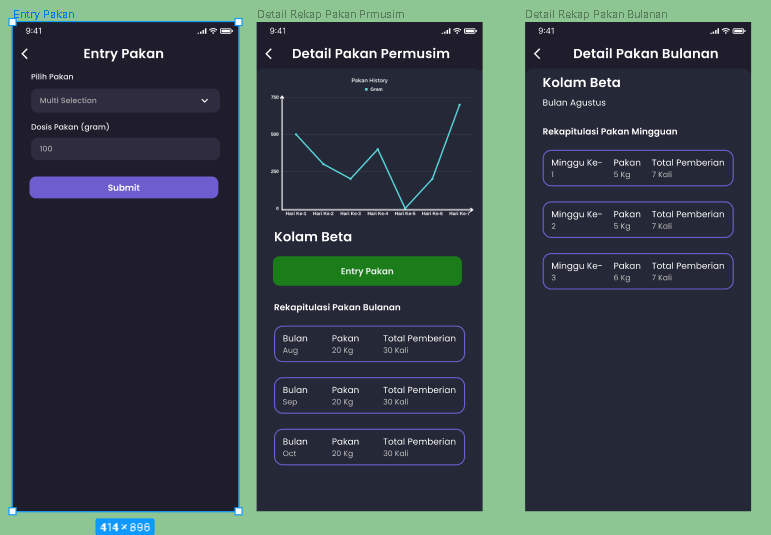
\includegraphics[keepaspectratio, width=4cm]{gambar/ssmockuppakan}
	\caption{\textit{Mock-up UI pemberian pakan}}
	\label{gambar:mockupsprint3}
	\end{figure}

	\item{\textit{Menerapkan mockup-UI  halaman pemberian pakan, rekapitulasi pakan kedalam code flutter}}
	
	Setelah \textit{mock-up UI  pemberian pakan, rekapitulasi pakan} dibuat, akan dilakukan pengimplementasian \textit{mock- up UI} ke dalam aplikasi menggukan flutter. Berikut adalah source code dari implementasi halaman  pemberian pakan, rekapitulasi pakan yang dikelompokan pada lampiran 4 dan menghasilkan output sebagai berikut.

	\begin{figure}[H]
	\centering
	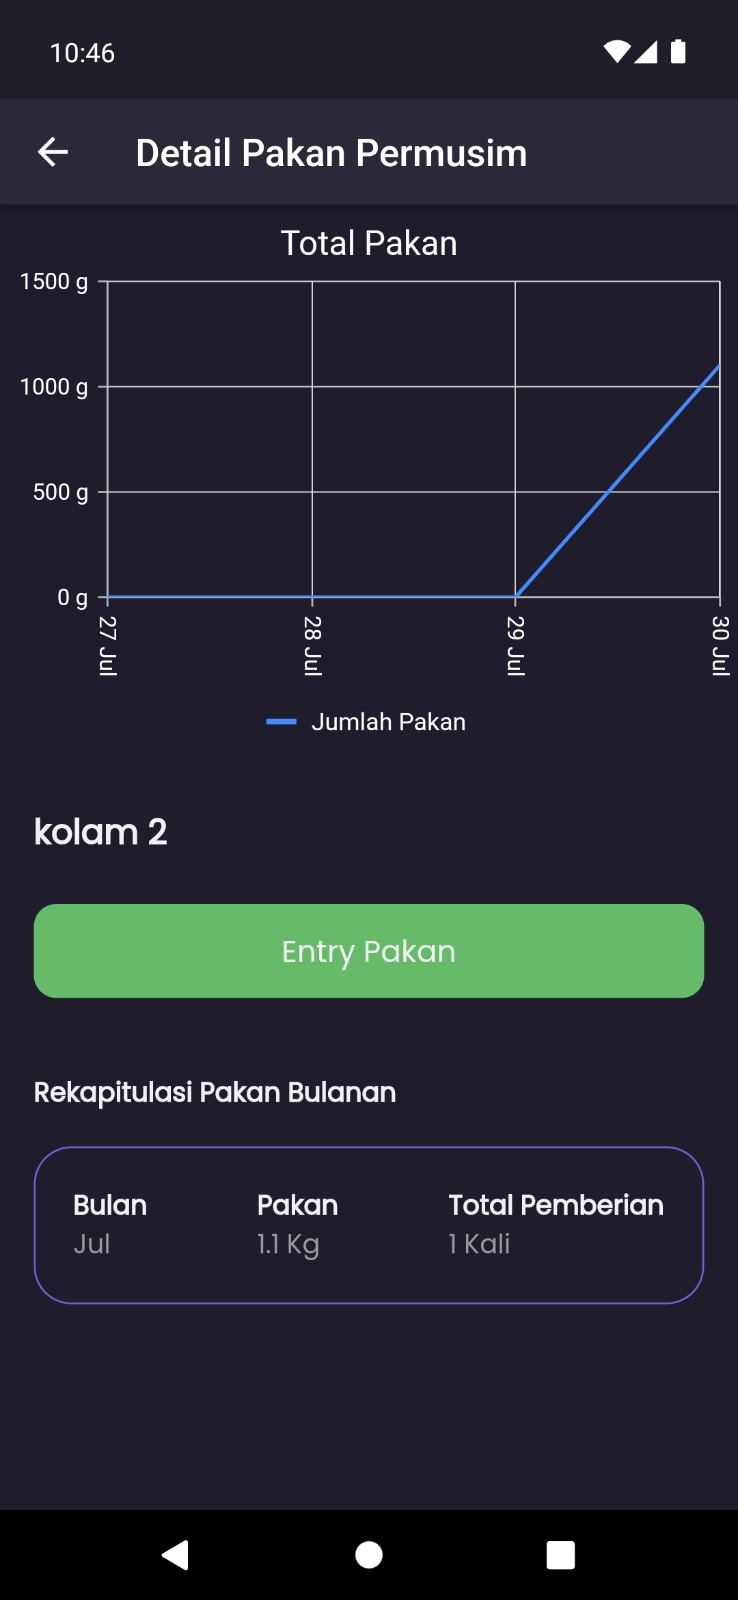
\includegraphics[keepaspectratio, width=3cm]{gambar/ssrekappakan}
	\caption{\textit{Output dari code pada rekapitulasi pakan}}
	\label{gambar:ssrekappakan}
	\end{figure}
	
	\begin{figure}[H]
	\centering
	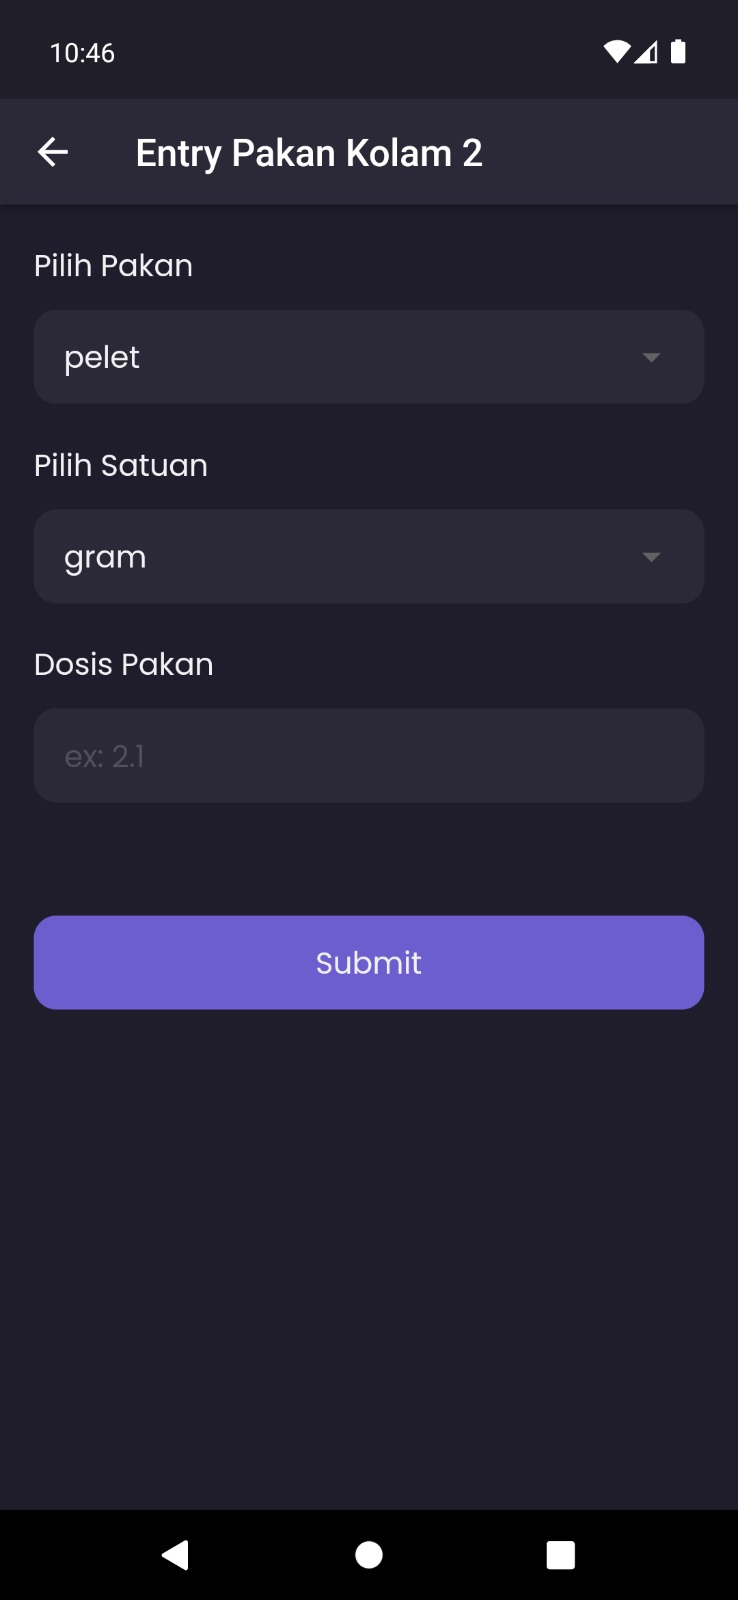
\includegraphics[keepaspectratio, width=4cm]{gambar/ssentrypakan}
	\caption{\textit{Output dari code untuk halaman entry pakan}}
	\label{gambar:ssentrypakan}
	\end{figure}

	\item{\textit{Mengitegrasikan fitur pemberian pakan dengan webservice}}

	Sebelumnya, setiap data pada fitur masih berupa data dummy sehingga perlu diintegrasikan dengan webservice agar aplikasi dapat berjalan dengan data yang asli. Hal yang dilakukan dalam mengintegrasikan fitur pemberian pakan dengan webservice terdapat pada lampiran 4.

  \item{Analisis \textit{User Experience}} 
 
Pada halaman pemberian pakan, pembudidaya harus memasukan dosis pakan dan jenis pakan yang diberikan sehingga data tersbut dapat diolah untuk output FCR nanti saat panen. Di halaman rekapitulasi pakan, terdapat grafik mengenai statistik jumlah pakan yang telah diberikan pada musim budidaya yang berjalan sehingga pembudidaya dapat dengan mudah mengetahui statistik rekap pakan dari setiap musim budidaya yang berjalan, selain itu terdapat juga list mengenai pakan yang telah diberikan yang berisi informasi dosis dan waktu pembudidaya saat memberikan pakan.


\item{Sprint 3 Review dan Sprint 4 Planning}

Sprint 3 diakhiri dengan melakukan weekly meeting pada hari selasa dengan agenda melakukan review dan testing terkait hasil sprint 3 dan melakukan planning untuk sprint 4 dengan rincian:
\begin{enumerate}
	\item{\textit{Review dan Testing hasil dari sprint 3}}

  Telah dilakukan review dan testing oleh penulis selaku developer dengan Scrum Master. Setelah dilakukan testing, Scrum Master menyimpulkan bahwa penerapan fitur pemberian pakan telah berjalan dengan baik.
  
\begin{longtable}{| p{8cm} | c | c | l |}
  \caption{Unit testing Halaman Daftar Kolam.\label{table:unit_testing_fitur_daftar_kolam}}\\
  \hline
  \multirow{2}{*}{Skenario Pengujian} & \multicolumn{2}{l|}{Kesesuaian} & \multirow{2}{*}{Kesimpulan} \\ 
  \cline{2-3}
    & \multicolumn{1}{l|}{sesuai} & tidak sesuai & \\ 
  \hline
  \hline
  \endfirsthead
  \hline
  \multirow{2}{*}{Skenario Pengujian} & \multicolumn{2}{l|}{Kesesuaian} & \multirow{2}{*}{Kesimpulan} \\ 
  \cline{2-3}
    & \multicolumn{1}{l|}{sesuai} & tidak sesuai &  \\ 
  \hline
  \hline
  \endhead
  \hline
  \endfoot
  
  
  \hline\hline
  \endlastfoot
   Saat ikon (+) ditekan maka akan menampilkan halaman registrasi kolam & \Checkmark &  & Diterima \\ 
  \hline
   Saat card kolam ditekan akan menampilkan halaman detail kolam & \Checkmark & & Diterima \\ 
  \hline
  \end{longtable}
  
  \begin{longtable}{| p{8cm} | c | c | l |}
  \caption{Unit testing Halaman Registrasi Kolam.\label{table:unit_testing_fitur_regis_kolam}}\\
  \hline
  \multirow{2}{*}{Skenario Pengujian} & \multicolumn{2}{l|}{Kesesuaian} & \multirow{2}{*}{Kesimpulan} \\ 
  \cline{2-3}
    & \multicolumn{1}{l|}{sesuai} & tidak sesuai & \\ 
  \hline
  \hline
  \endfirsthead
  \hline
  \multirow{2}{*}{Skenario Pengujian} & \multicolumn{2}{l|}{Kesesuaian} & \multirow{2}{*}{Kesimpulan} \\ 
  \cline{2-3}
    & \multicolumn{1}{l|}{sesuai} & tidak sesuai &  \\ 
  \hline
  \hline
  \endhead
  \hline
  \endfoot
  
  
  \hline\hline
  \endlastfoot
   ketika mengisi form registrasi kolam dengan data yang sesuai dan menekan submit, maka kolam baru akan ditambakan & \Checkmark &  & Diterima \\ 
  \hline
  \end{longtable}
  
  \begin{longtable}{| p{8cm} | c | c | l |}
  \caption{Unit testing Halaman Detail Kolam.\label{table:unit_testing_fitur_detail_kolam}}\\
  \hline
  \multirow{2}{*}{Skenario Pengujian} & \multicolumn{2}{l|}{Kesesuaian} & \multirow{2}{*}{Kesimpulan} \\ 
  \cline{2-3}
    & \multicolumn{1}{l|}{sesuai} & tidak sesuai & \\ 
  \hline
  \hline
  \endfirsthead
  \hline
  \multirow{2}{*}{Skenario Pengujian} & \multicolumn{2}{l|}{Kesesuaian} & \multirow{2}{*}{Kesimpulan} \\ 
  \cline{2-3}
    & \multicolumn{1}{l|}{sesuai} & tidak sesuai &  \\ 
  \hline
  \hline
  \endhead
  \hline
  \endfoot
  
  
  \hline\hline
  \endlastfoot
   ketika tombol kualitas air ditekan maka akan menampilkan halaman kualitas air & \Checkmark &  & Diterima \\ 
  \hline
   ketikan menekan salah satu list dari masa budidaya akan menampilkan halaman detail masa budidaya & \Checkmark &  & Diterima \\ 
  \hline
   ketika status kolam tidak aktif atau panen dan menekan tombol start budidaya, maka akan menampilkan halaman aktivasi kolam & \Checkmark &  & Diterima \\ 
  \hline
   ketika status kolam aktif dan menekan tombol aktif, maka akan menampilkan halaman deaktivasi kolam & \Checkmark &  & Diterima \\ 
  \hline
  \end{longtable}
  
  \begin{longtable}{| p{8cm} | c | c | l |}
  \caption{Unit testing Halaman Registrasi Kolam.\label{table:unit_testing_fitur_regis_kolam}}\\
  \hline
  \multirow{2}{*}{Skenario Pengujian} & \multicolumn{2}{l|}{Kesesuaian} & \multirow{2}{*}{Kesimpulan} \\ 
  \cline{2-3}
    & \multicolumn{1}{l|}{sesuai} & tidak sesuai & \\ 
  \hline
  \hline
  \endfirsthead
  \hline
  \multirow{2}{*}{Skenario Pengujian} & \multicolumn{2}{l|}{Kesesuaian} & \multirow{2}{*}{Kesimpulan} \\ 
  \cline{2-3}
    & \multicolumn{1}{l|}{sesuai} & tidak sesuai &  \\ 
  \hline
  \hline
  \endhead
  \hline
  \endfoot
  
  
  \hline\hline
  \endlastfoot
   ketika mengisi form registrasi kolam dengan data yang sesuai dan menekan submit, maka kolam baru akan ditambakan & \Checkmark &  & Diterima \\ 
  \hline
  \end{longtable}
  
  \begin{longtable}{| p{8cm} | c | c | l |}
  \caption{Unit testing Halaman Aktivasi Kolam.\label{table:unit_testing_fitur_aktivasi_kolam}}\\
  \hline
  \multirow{2}{*}{Skenario Pengujian} & \multicolumn{2}{l|}{Kesesuaian} & \multirow{2}{*}{Kesimpulan} \\ 
  \cline{2-3}
    & \multicolumn{1}{l|}{sesuai} & tidak sesuai & \\ 
  \hline
  \hline
  \endfirsthead
  \hline
  \multirow{2}{*}{Skenario Pengujian} & \multicolumn{2}{l|}{Kesesuaian} & \multirow{2}{*}{Kesimpulan} \\ 
  \cline{2-3}
    & \multicolumn{1}{l|}{sesuai} & tidak sesuai &  \\ 
  \hline
  \hline
  \endhead
  \hline
  \endfoot
  
  
  \hline\hline
  \endlastfoot
   ketika mengisi form aktivasi kolam dengan data yang sesuai dan menekan submit, maka musim budidaya baru akan ditambahkan dan status kolam menjadi aktif & \Checkmark &  & Diterima \\ 
  \hline
  \end{longtable}
  
  \begin{longtable}{| p{8cm} | c | c | l |}
  \caption{Unit testing Halaman Deaktivasi Kolam.\label{table:unit_testing_fitur_deaktivasi_kolam}}\\
  \hline
  \multirow{2}{*}{Skenario Pengujian} & \multicolumn{2}{l|}{Kesesuaian} & \multirow{2}{*}{Kesimpulan} \\ 
  \cline{2-3}
    & \multicolumn{1}{l|}{sesuai} & tidak sesuai & \\ 
  \hline
  \hline
  \endfirsthead
  \hline
  \multirow{2}{*}{Skenario Pengujian} & \multicolumn{2}{l|}{Kesesuaian} & \multirow{2}{*}{Kesimpulan} \\ 
  \cline{2-3}
    & \multicolumn{1}{l|}{sesuai} & tidak sesuai &  \\ 
  \hline
  \hline
  \endhead
  \hline
  \endfoot
  
  
  \hline\hline
  \endlastfoot
   ketika mengisi form deaktivasi kolam dengan data yang sesuai dan menekan submit, maka musim budidaya yang barjalan akan berhenti status kolam menjadi tidak aktif & \Checkmark &  & Diterima \\ 
  \hline
  \end{longtable}
  

  \begin{longtable}{| p{8cm} | c | c | l |}
    \caption{Unit testing Halaman Detail Masa Budidaya.\label{table:unit_testing_detail_budidaya}}\\
    \hline
    \multirow{2}{*}{Skenario Pengujian} & \multicolumn{2}{l|}{Kesesuaian} & \multirow{2}{*}{Kesimpulan} \\ 
    \cline{2-3}
      & \multicolumn{1}{l|}{sesuai} & tidak sesuai & \\ 
    \hline
    \hline
    \endfirsthead
    \hline
    \multirow{2}{*}{Skenario Pengujian} & \multicolumn{2}{l|}{Kesesuaian} & \multirow{2}{*}{Kesimpulan} \\ 
    \cline{2-3}
      & \multicolumn{1}{l|}{sesuai} & tidak sesuai &  \\ 
    \hline
    \hline
    \endhead
    \hline
    \endfoot
    
    
    \hline\hline
    \endlastfoot
    Ketika tombol rekapitulasi pakan ditekan, maka akan ditampilkan halaman rekapitulasi pakan & \Checkmark &  & Diterima \\ 
    \hline
    Ketika tombol rekapitulasi kematian ikan ditekan, maka akan ditampilkan halaman rekapitulasi kematian ikan & \Checkmark &  & Diterima \\ 
    \hline
    Ketika tombol rekapitulasi grading ikan ditekan, maka akan ditampilkan halaman rekapitulasi grading ikan & \Checkmark &  & Diterima \\ 
    \hline
    Ketika tombol treatment ditekan, maka akan ditampilkan halaman treatment kolam & \Checkmark &  & Diterima \\ 
    \hline
     Ketika tombol sortir ditekan, maka akan ditampilkan halaman sortir kolam & \Checkmark &  & Diterima \\ 
    \hline
    \end{longtable}
    
    
    \begin{longtable}{| p{8cm} | c | c | l |}
    \caption{Unit testing Halaman Rekapitulasi Pakan.\label{table:unit_testing_rekapitulasi_pakan}}\\
    \hline
    \multirow{2}{*}{Skenario Pengujian} & \multicolumn{2}{l|}{Kesesuaian} & \multirow{2}{*}{Kesimpulan} \\ 
    \cline{2-3}
      & \multicolumn{1}{l|}{sesuai} & tidak sesuai & \\ 
    \hline
    \hline
    \endfirsthead
    \hline
    \multirow{2}{*}{Skenario Pengujian} & \multicolumn{2}{l|}{Kesesuaian} & \multirow{2}{*}{Kesimpulan} \\ 
    \cline{2-3}
      & \multicolumn{1}{l|}{sesuai} & tidak sesuai &  \\ 
    \hline
    \hline
    \endhead
    \hline
    \endfoot
    
    
    \hline\hline
    \endlastfoot
    Ketika menekan list data rekapitulasi pakan, maka akan ditamplikan detail rekapitulasi pakan & \Checkmark &  & Diterima \\ 
    \hline
    Ketika menekan list data rekapitulasi pakan, maka akan ditamplikan detail rekapitulasi pakan & \Checkmark &  & Diterima \\ 
    \hline
    Saat tombol entry pakan ditekan maka akan menampilkan halaman entry pakan & \Checkmark &  & Diterima \\ 
    \hline
     ketika mengisi form rekapitulasi pakan dengan data yang sesuai dan menekan submit, data rekapitulasi pakan akan ditambahkan & \Checkmark &  & Diterima \\ 
    \hline
    \end{longtable}

	\item{\textit{Sprint Planning untuk Sprint 4}}
	
	Planning untuk sprint 4 yakni membuat fitur grading ikan pada aplikasi \textit{Assistive Aquaculture Breeding Management}.
\end{enumerate}
\end{enumerate}
%!TEX root = ./template-skripsi.tex

\subsection{\textit{Sprint 4}}

	\textit{Sprint-4} dilakukan sepekan pada tanggal 13 September 2022 sampai dengan 20 september 2022. \textit{Story} keempat pada \textit{product backlog} yaitu membuat grading berat dipecah menjadi beberapa \textit{task} sebagai berikut.


 \begin{longtable}[c]{@{} |p{1cm}|p{4cm}|p{5cm}|p{3cm}| @{}}
 \caption{\textit{Sprint 4} \label{sprint4_table}}\\


 \hline
  \multirow{1}{=}{\centering{\textbf{No}}} & \multirow{1}{=}{\centering{\textbf{\textit{Story}}}} & \multirow{1}{=}{\centering{\textbf{\textit{Task}}}} & \multirow{1}{=}{\centering{\textbf{\textit{Status}}}}\\
 \endfirsthead

 \hline
  \multirow{1}{=}{\centering{\textbf{No}}} & \multirow{1}{=}{\centering{\textbf{\textit{Story}}}} & \multirow{1}{=}{\centering{\textbf{\textit{Task}}}} & \multirow{1}{=}{\centering{\textbf{\textit{Status}}}}\\
 \endhead

 \hline
 \endfoot

 \hline
 \endlastfoot

 \hline
 1 & Membuat fitur grading berat ikan &  Membuat \textit{Mock-up UI} halaman rekapitulasi grading, detail grading, entry grading  &  selesai \\
 \hline
 2 & & Menerapkan \textit{Mock-up UI} halaman rekapitulasi grading, detail grading, entry grading ke Flutter & selesai\\
 \hline
 3 & & Mengintegrasikan halaman rekapitulasi grading, detail grading, entry grading ke \textit{webservice} & selesai\\
 \hline
 \end{longtable}

Pada sprint keempat ini story yang di pilih untuk di uraikan pada sprint kali ini adalah membuat halaman rekapitulasi grading, detail grading, entry grading. Tujuan dari \textit{sprint-4} ini adalah membuat fitur grading berat ikan dan mengintegrasikan halaman tersebut dengan webservice yang sudah dibuat oleh penelitian Andri Rahmanto.

\begin{enumerate}[listparindent=2em]
	
	\item{\textit{Membuat Mock-up UI Fitur Grading}}
	
	Pembuatan konten dan fitur yang terdapat pada \textit{mock-up UI} fitur grading dilakukan berdasarkan persetujuan product owner dan scrum master pada meeting sebelumnya. Mock-up UI dibuat menggunakan platform figma.
	
	\begin{figure}[H]
	\centering
	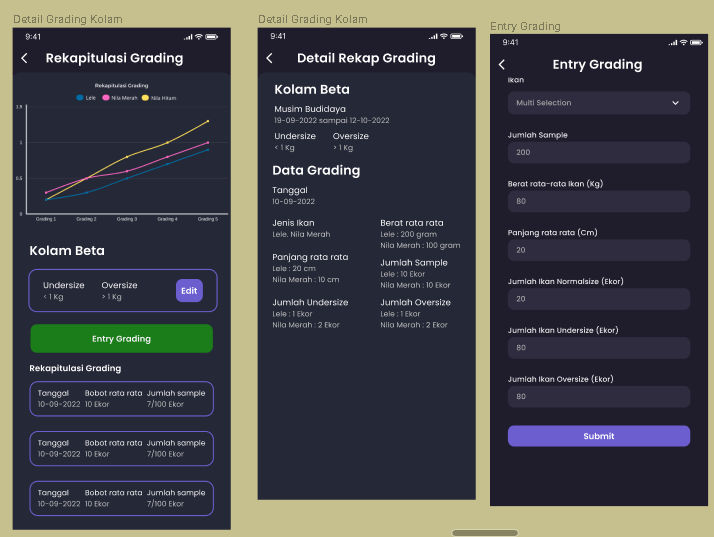
\includegraphics[keepaspectratio, width=6cm]{gambar/mockupgrading}
	\caption{\textit{Mock-up UI Fitur Grading}}
	\label{gambar:mockupgrading}
	\end{figure}

	\item{\textit{Class Diagram}}
	
	Class Diagram menggambarkan kelas-kelas yang akan dipakai oleh sistem. Umumnya terdapat 3 kelas pada setiap module yaitu class model, controller, dan view. Pada sprint-4 penelitian kali ini penulis membuat 4 class yaitu model yang berwarna biru, view berwarna oranye, controller yang berwarna hijau, dan service yang berwarna kuning.
	 
	 \begin{figure}[H]
	 \centering
	 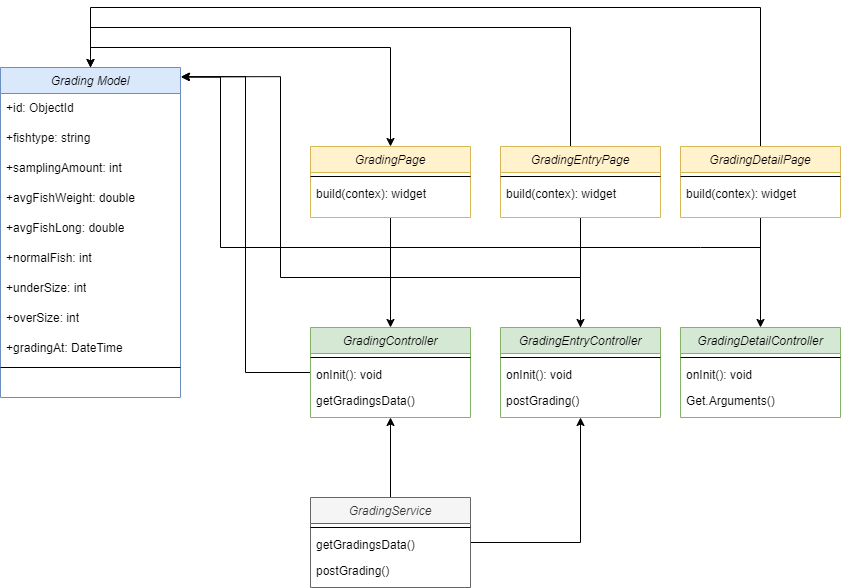
\includegraphics[keepaspectratio, width=6cm]{gambar/gradingcd}
	 \caption{\textit{Class Diagram Fitur Sprint-4}}
	 \label{gambar:gradingcd}
	 \end{figure}


	\item{\textit{Menerapkan Mockup-UI Fitur Grading kedalam code flutter}}
	
	Setelah \textit{mock-up UI fitur grading} hingga prototype dibuat, akan dilakukan pengimplementasian \textit{mock-up UI} ke dalam aplikasi menggukan flutter. Source code dari implementasi fitur grading terdapat pada lampiran 5 yang menghasilkan output halaman sebagai berikut
	
	\begin{figure}[H]
		\centering
		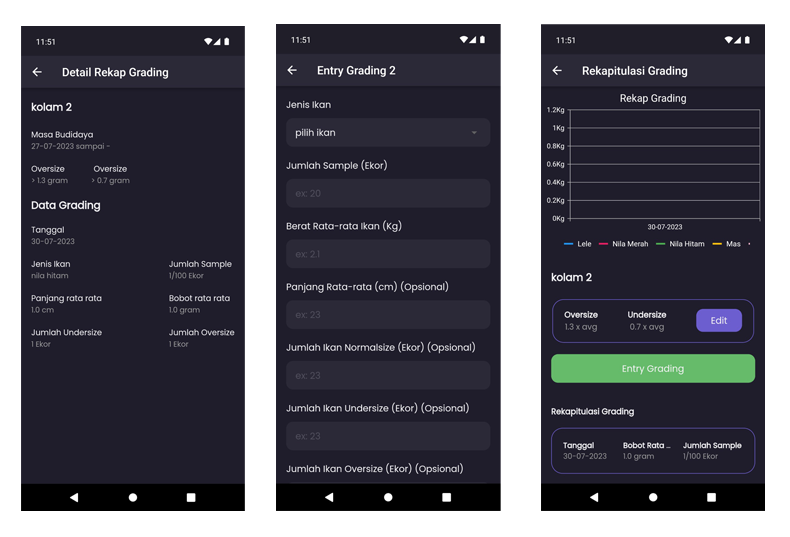
\includegraphics[keepaspectratio, width=8cm]{gambar/sssprint4}
		\caption{\textit{Output dari code pada sprint 4}}
		\label{gambar:sssprint4}
		\end{figure}

	\item{\textit{Mengitegrasikan fitur grading dengan webservice}}

	Sebelumnya, setiap data pada fitur masih berupa data dummy sehingga perlu diintegrasikan dengan webservice agar aplikasi dapat berjalan dengan data yang asli. Hal yang dilakukan dalam mengintegrasikan fitur grading dengan webservice terdapat pada lampiran 5.
	
  \item{Analisis \textit{User Experience}} 
 
  Pada halaman grading, pembudidaya harus jenis ikan dan data klasifikasi ukuran ikan. Di halaman rekapitulasi grading, terdapat grafik mengenai statistik pertumbuhan ikan  pada musim budidaya yang berjalan sehingga pembudidaya dapat dengan mudah mengetahui perkembangan ukuran ikan dari waktu ke waktu, selain itu terdapat juga list mengenai grading yang telah dilakukan yang berisi informasi yang berhubungan dengan ukuran ikan saat dilakukan grading.

\item{Sprint 4 Review dan Sprint 5 Planning}

Sprint 4 diakhiri dengan melakukan weekly meeting pada hari selasa dengan agenda melakukan review dan testing terkait hasil sprint 4 dan melakukan planning untuk sprint 5 dengan rincian:
\begin{enumerate}
	\item{\textit{Review dan Testing hasil dari sprint 4}}

	Telah dilakukan review dan testing oleh penulis selaku developer dengan Scrum Master. Setelah dilakukan testing, Scrum Master menyimpulkan bahwa fitur grading berat ikan telah berjalan dengan baik.
\begin{longtable}{| p{8cm} | c | c | l |}
  \caption{Unit testing Halaman Rekapitulasi Grading.\label{table:unit_testing_rekapitulasi_grading}}\\
  \hline
  \multirow{2}{*}{Skenario Pengujian} & \multicolumn{2}{l|}{Kesesuaian} & \multirow{2}{*}{Kesimpulan} \\ 
  \cline{2-3}
    & \multicolumn{1}{l|}{sesuai} & tidak sesuai & \\ 
  \hline
  \hline
  \endfirsthead
  \hline
  \multirow{2}{*}{Skenario Pengujian} & \multicolumn{2}{l|}{Kesesuaian} & \multirow{2}{*}{Kesimpulan} \\ 
  \cline{2-3}
    & \multicolumn{1}{l|}{sesuai} & tidak sesuai &  \\ 
  \hline
  \hline
  \endhead
  \hline
  \endfoot
  
  
  \hline\hline
  \endlastfoot
  Ketika menekan list data rekapitulasi grading, maka akan ditamplikan detail rekapitulasi grading & \Checkmark &  & Diterima \\ 
  \hline
  Ketika menekan list data rekapitulasi grading, maka akan ditamplikan detail rekapitulasi grading & \Checkmark &  & Diterima \\ 
  \hline
  Saat tombol entry grading ditekan maka akan menampilkan halaman entry grading & \Checkmark &  & Diterima \\ 
  \hline
  ketika mengisi form rekapitulasi grading dengan data yang sesuai dan menekan submit, data rekapitulasi grading akan ditambahkan & \Checkmark &  & Diterima \\ 
  \hline
  \end{longtable}

	\item{\textit{Sprint Planning untuk Sprint 5}}
	
	Planning untuk sprint 5 yakni membuat fitur rekapitulasi kematian ikan pada aplikasi \textit{Assistive Aquaculture Breeding Management}.
\end{enumerate}
\end{enumerate}	
%!TEX root = ./template-skripsi.tex

\subsection{\textit{Sprint 5}}

	\textit{Sprint-5} dilakukan sepekan pada tanggal 20 September 2022 sampai dengan 27 september 2022. \textit{Story} kelimat pada \textit{product backlog} yaitu membuat fitur rekapitulasi kematian ikan dipecah menjadi beberapa \textit{task} sebagai berikut.


 \begin{longtable}[c]{@{} |p{1cm}|p{4cm}|p{5cm}|p{3cm}| @{}}
 \caption{\textit{Sprint 5} \label{sprint5_table}}\\


 \hline
  \multirow{1}{=}{\centering{\textbf{No}}} & \multirow{1}{=}{\centering{\textbf{\textit{Story}}}} & \multirow{1}{=}{\centering{\textbf{\textit{Task}}}} & \multirow{1}{=}{\centering{\textbf{\textit{Status}}}}\\
 \endfirsthead

 \hline
  \multirow{1}{=}{\centering{\textbf{No}}} & \multirow{1}{=}{\centering{\textbf{\textit{Story}}}} & \multirow{1}{=}{\centering{\textbf{\textit{Task}}}} & \multirow{1}{=}{\centering{\textbf{\textit{Status}}}}\\
 \endhead

 \hline
 \endfoot

 \hline
 \endlastfoot

 \hline
 1 & Membuat fitur rekapitulasi kematian ikan &  Membuat \textit{Mock-up UI} halaman rekapitulasi kematian ikan, entry kematian ikan  &  selesai \\
 \hline
 2 & & Menerapkan \textit{Mock-up UI} halaman rekapitulasi kematian ikan, entry kematian ikan ke Flutter & selesai\\
 \hline
 3 & & Mengintegrasikan halaman rekapitulasi kematian ikan, entry kematian ikan ke \textit{webservice} & selesai\\
 \hline
 \end{longtable}

Pada sprint kelima ini story yang di pilih untuk di uraikan pada sprint kali ini adalah membuat halaman rekapitulasi kematian ikan, entry kematian ikan. Tujuan dari \textit{sprint-5} ini adalah membuat fitur rekapitulasi kematian ikan dan mengintegrasikan halaman tersebut dengan webservice yang sudah dibuat oleh penelitian Andri Rahmanto.

\begin{enumerate}[listparindent=2em]
	
	\item{\textit{Membuat Mock-up UI Fitur Rekapitulasi Kematian Ikan}}
	
	Pembuatan konten dan fitur yang terdapat pada \textit{mock-up UI} fitur rekapitulasi kematian ikan dilakukan berdasarkan persetujuan product owner dan scrum master pada meeting sebelumnya. Mock-up UI dibuat menggunakan platform figma.
	
	\begin{figure}[H]
	\centering
	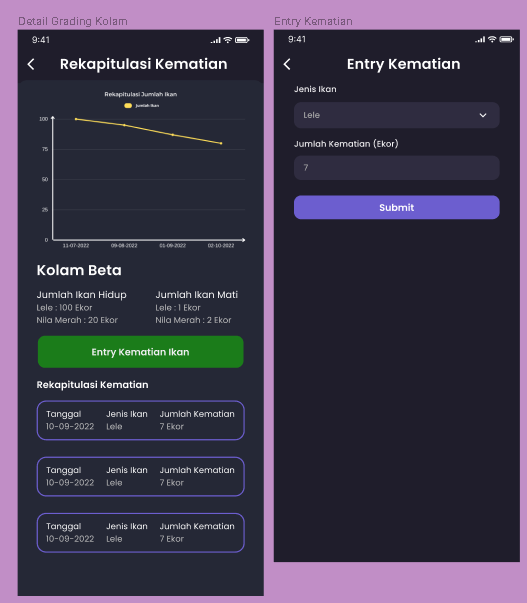
\includegraphics[keepaspectratio, width=6cm]{gambar/mockupkematian}
	\caption{\textit{Mock-up UI Fitur Rekapitulasi Kematian Ikan}}
	\label{gambar:mockupkematian}
	\end{figure}

	\item{\textit{Class Diagram}}
	
	Class Diagram menggambarkan kelas-kelas yang akan dipakai oleh sistem. Umumnya terdapat 3 kelas pada setiap module yaitu class model, controller, dan view. Pada sprint-5 penelitian kali ini penulis membuat 4 class yaitu model yang berwarna biru, view berwarna oranye, controller yang berwarna hijau, dan service yang berwarna kuning.
	 
	 \begin{figure}[H]
	 \centering
	 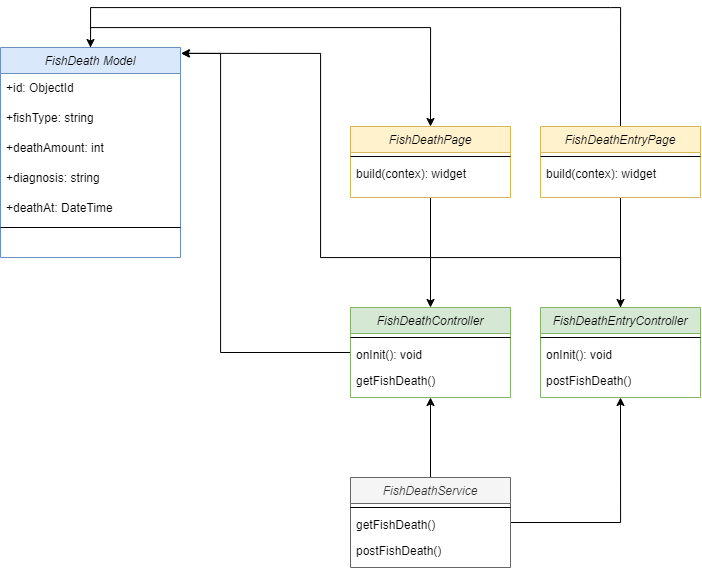
\includegraphics[keepaspectratio, width=6cm]{gambar/deathcd}
	 \caption{\textit{Class Diagram Fitur Sprint-5}}
	 \label{gambar:deathcd}
	 \end{figure}

	\item{\textit{Menerapkan Mockup-UI fitur rekapitulasi kematian ikan kedalam code flutter}}
	
	Setelah itu, akan dilakukan pengimplementasian \textit{mock-up UI} ke dalam aplikasi menggukan flutter. Pada lampiran 6 source code dari implementasi fitur grading yang dikelompokan berdasarkan halaman yang menghasilkan output halaman seperti dibawah ini.

	\begin{figure}[H]
		\centering
		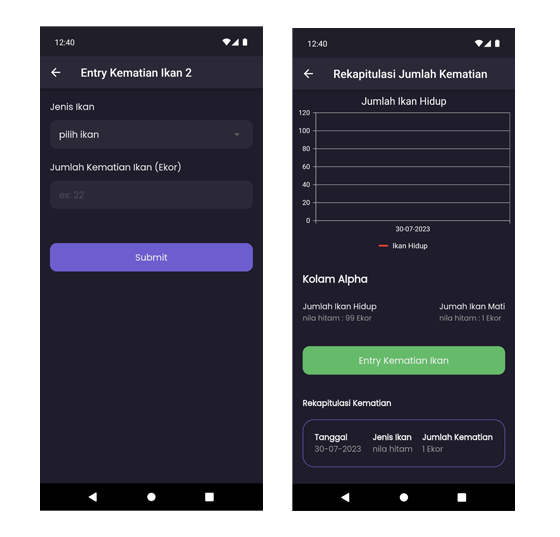
\includegraphics[keepaspectratio, width=8cm]{gambar/sssprint5}
		\caption{\textit{Output dari code pada sprint 5}}
		\label{gambar:sssprint5}
		\end{figure}

	\item{\textit{Mengitegrasikan fitur rekapitulasi kematian dengan webservice}}

	Sebelumnya, setiap data pada fitur masih berupa data dummy sehingga perlu diintegrasikan dengan webservice agar aplikasi dapat berjalan dengan data yang asli. Hal yang dilakukan dalam mengintegrasikan fitur rekapitulasi kematian ikan dengan webservice terdapat pada lampiran 6.

  \item{Analisis \textit{User Experience}} 
 
  Pada halaman entry rekapitulasi kematian, pembudidaya harus jenis ikan dan data jumlah kematian. Di halaman rekapitulasi kematian, terdapat grafik mengenai statistik jumlah ikan  pada musim budidaya yang berjalan sehingga pembudidaya dapat dengan mudah mengetahui penurunan jumlah ikan akibat kematian. Selain itu terdapat juga list mengenai data kematian yang telah dimasukan yang berisi informasi yang berhubungan dengan kematian ikan.

\item{Sprint 5 Review dan Sprint 6 Planning}

Sprint 5 diakhiri dengan melakukan weekly meeting pada hari selasa dengan agenda melakukan review dan testing terkait hasil sprint 5 dan melakukan planning untuk sprint 6 dengan rincian:
\begin{enumerate}
	\item{\textit{Review dan Testing hasil dari sprint 5}}

	Telah dilakukan review dan testing oleh penulis selaku developer dengan Scrum Master. Setelah dilakukan testing, Scrum Master menyimpulkan bahwa fitur rekapitulasi kematian ikan telah berjalan dengan baik.
	
  \begin{longtable}{| p{8cm} | c | c | l |}
    \caption{Unit testing Halaman Rekapitulasi Kematian.\label{table:unit_testing_rekapitulasi_kematian}}\\
    \hline
    \multirow{2}{*}{Skenario Pengujian} & \multicolumn{2}{l|}{Kesesuaian} & \multirow{2}{*}{Kesimpulan} \\ 
    \cline{2-3}
      & \multicolumn{1}{l|}{sesuai} & tidak sesuai & \\ 
    \hline
    \hline
    \endfirsthead
    \hline
    \multirow{2}{*}{Skenario Pengujian} & \multicolumn{2}{l|}{Kesesuaian} & \multirow{2}{*}{Kesimpulan} \\ 
    \cline{2-3}
      & \multicolumn{1}{l|}{sesuai} & tidak sesuai &  \\ 
    \hline
    \hline
    \endhead
    \hline
    \endfoot
    
    
    \hline\hline
    \endlastfoot
    Ketika menekan list data rekapitulasi pakan, maka akan ditamplikan detail rekapitulasi pakan & \Checkmark &  & Diterima \\ 
    \hline
    Saat tombol entry kematian ditekan maka akan menampilkan halaman entry kematian & \Checkmark &  & Diterima \\ 
    \hline
    ketika mengisi form rekapitulasi kematian dengan data yang sesuai dan menekan submit, data rekapitulasi kematian akan ditambahkan & \Checkmark &  & Diterima \\ 
    \hline
    \end{longtable}

	\item{\textit{Sprint Planning untuk Sprint 6}}
	
	Planning untuk sprint 6 yakni membuat fitur treatment kolam pada aplikasi \textit{Assistive Aquaculture Breeding Management}.
\end{enumerate}
\end{enumerate}
%!TEX root = ./template-skripsi.tex

\subsection{\textit{Sprint 6}}

	\textit{Sprint-6} dilakukan sepekan pada tanggal 27 September 2022 sampai dengan 4 oktober 2022. \textit{Story} keenam pada \textit{product backlog} yaitu membuat fitur treatment kolam dipecah menjadi beberapa \textit{task} sebagai berikut.


 \begin{longtable}[c]{@{} |p{1cm}|p{4cm}|p{5cm}|p{3cm}| @{}}
 \caption{\textit{Sprint 6} \label{sprint6_table}}\\


 \hline
  \multirow{1}{=}{\centering{\textbf{No}}} & \multirow{1}{=}{\centering{\textbf{\textit{Story}}}} & \multirow{1}{=}{\centering{\textbf{\textit{Task}}}} & \multirow{1}{=}{\centering{\textbf{\textit{Status}}}}\\
 \endfirsthead

 \hline
  \multirow{1}{=}{\centering{\textbf{No}}} & \multirow{1}{=}{\centering{\textbf{\textit{Story}}}} & \multirow{1}{=}{\centering{\textbf{\textit{Task}}}} & \multirow{1}{=}{\centering{\textbf{\textit{Status}}}}\\
 \endhead

 \hline
 \endfoot

 \hline
 \endlastfoot

 \hline
 1 & Membuat fitur treatment kolam &  Membuat \textit{Mock-up UI} halaman list treatment, detail treatment, entry treatment &  selesai \\
 \hline
 2 & & Menerapkan \textit{Mock-up UI} halaman list treatment, detail treatment, entry treatment  ke Flutter & selesai\\
 \hline
 \end{longtable}

Pada sprint keenam ini story yang di pilih untuk di uraikan pada sprint kali ini adalah membuat halaman rekapitulasi treatment, detail treatment, entry treatment. Tujuan dari \textit{sprint-6} ini adalah membuat fitur treatment berat ikan dan mengintegrasikan halaman tersebut dengan webservice yang sudah dibuat oleh penelitian Andri Rahmanto.
	


\begin{enumerate}[listparindent=2em]
	
	\item{\textit{Membuat Mock-up UI Fitur Treatment Kolam}}
	
	Pembuatan konten dan fitur yang terdapat pada \textit{mock-up UI} fitur treatment kolam dilakukan berdasarkan persetujuan product owner dan scrum master pada meeting sebelumnya. Mock-up UI dibuat menggunakan platform figma.
	
	\begin{figure}[H]
	\centering
	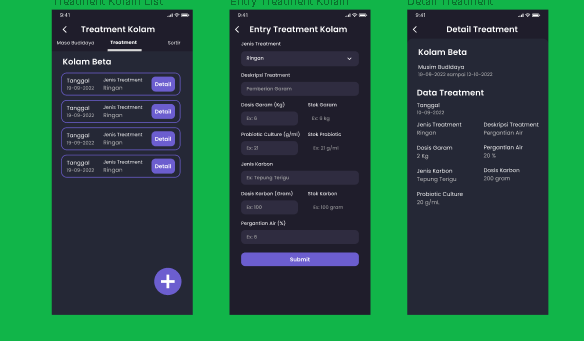
\includegraphics[keepaspectratio, width=6cm]{gambar/mockuptreatment}
	\caption{\textit{Mock-up UI Fitur treatment}}
	\label{gambar:mockuptreatment}
	\end{figure}

	\item{\textit{Class Diagram}}
	
	Class Diagram menggambarkan kelas-kelas yang akan dipakai oleh sistem. Umumnya terdapat 3 kelas pada setiap module yaitu class model, controller, dan view. Pada sprint-6 penelitian kali ini penulis membuat 4 class yaitu model yang berwarna biru, view berwarna oranye, controller yang berwarna hijau, dan service yang berwarna kuning.
	 
	 \begin{figure}[H]
	 \centering
	 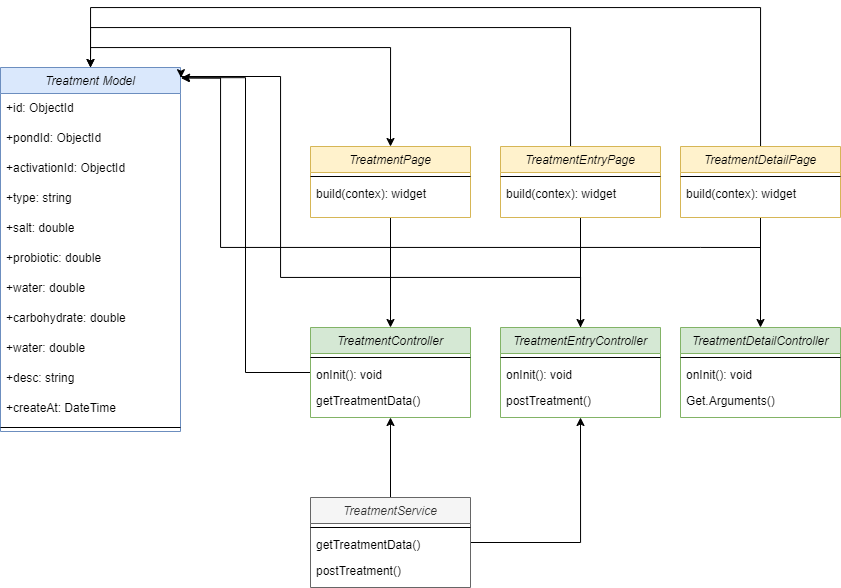
\includegraphics[keepaspectratio, width=6cm]{gambar/treatmentcd}
	 \caption{\textit{Class Diagram Fitur Sprint-6}}
	 \label{gambar:treatmentcd}
	 \end{figure}

	\item{\textit{Menerapkan Mockup-UI Fitur Treatment Kolam kedalam code flutter}}
	
	Setelah \textit{mock-up UI fitur treatment kolam}, akan dilakukan pengimplementasian \textit{mock-up UI} ke dalam aplikasi menggukan flutter. Pada lampiran 7 terdapat source code dari implementasi fitur treatment yang dikelompokan berdasarkan halaman yang menghasilkan halaman seperti dibawah ini.
	
	\begin{figure}[H]
		\centering
		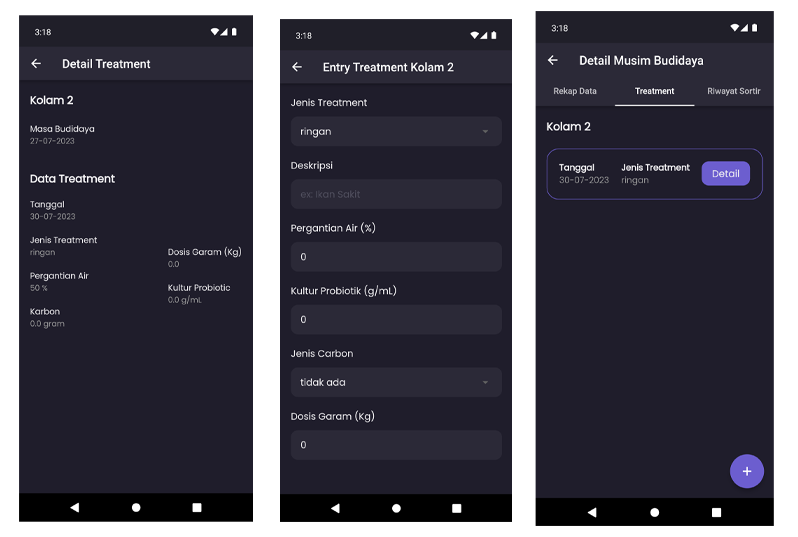
\includegraphics[keepaspectratio, width=8cm]{gambar/sssprint6}
		\caption{\textit{Output dari code pada sprint 6}}
		\label{gambar:sssprint6}
		\end{figure}

  \item{Analisis \textit{User Experience}} 
 
  Pada halaman entry treatment, pembudidaya harus memasukan data yang diperlukan untuk melakukan treatment kolam sesuai dengan kesepakatan saat meeting. Selain itu terdapat juga list mengenai data treatment yang telah dimasukan yang berisi informasi yang berhubungan dengan treatment kolam. Terdapat pula halaman detail treatment yang berisi informasi yang lebih detail terkait treatment yang telah dilakukan.

\item{Sprint 6 Review dan Sprint 7 Planning}

Sprint 6 diakhiri dengan melakukan weekly meeting pada hari selasa dengan agenda melakukan review dan testing terkait hasil sprint 6 dan melakukan planning untuk sprint 7 dengan rincian:
\begin{enumerate}
	\item{\textit{Review dan Testing hasil dari sprint 6}}

	Telah dilakukan review dan testing oleh penulis selaku developer dengan Scrum Master. Setelah dilakukan testing, Scrum Master menyimpulkan bahwa fitur treatment kolam telah berjalan dengan baik.

	\item{\textit{Sprint Planning untuk Sprint 7}}
	
	Planning untuk sprint 7 yakni membuat halaman untuk fitur treatment kolam pada aplikasi \textit{Assistive Aquaculture Breeding Management}.
\end{enumerate}
\end{enumerate}
%!TEX root = ./template-skripsi.tex

\subsection{\textit{Sprint 8}}

	\textit{Sprint-8} dilakukan sepekan pada tanggal 4 oktober 2022 sampai dengan 11 oktober 2022. \textit{Story} ketujuh pada \textit{product backlog} yaitu mengintegrasikan fitur treatment kolam dipecah menjadi beberapa \textit{task} sebagai berikut.


 \begin{longtable}[c]{@{} |p{1cm}|p{4cm}|p{5cm}|p{3cm}| @{}}
 \caption{\textit{Sprint 7} \label{sprint7_table}}\\


 \hline
  \multirow{1}{=}{\centering{\textbf{No}}} & \multirow{1}{=}{\centering{\textbf{\textit{Story}}}} & \multirow{1}{=}{\centering{\textbf{\textit{Task}}}} & \multirow{1}{=}{\centering{\textbf{\textit{Status}}}}\\
 \endfirsthead

 \hline
  \multirow{1}{=}{\centering{\textbf{No}}} & \multirow{1}{=}{\centering{\textbf{\textit{Story}}}} & \multirow{1}{=}{\centering{\textbf{\textit{Task}}}} & \multirow{1}{=}{\centering{\textbf{\textit{Status}}}}\\
 \endhead

 \hline
 \endfoot

 \hline
 \endlastfoot

 \hline
 1 & Mengitegrasikan fitur treatment kolam dengan webservice &  Mengitegrasikan fitur treatment kolam dengan webservice &  selesai \\
 \hline
 \end{longtable}

Pada sprint ketujuh ini story yang di pilih untuk di uraikan pada sprint kali ini adalah membuat halaman rekapitulasi treatment kolam, entry treatment kolam. Tujuan dari \textit{sprint-7} ini adalah membuat fitur rekapitulasi treatment kolam dan mengintegrasikan halaman tersebut dengan webservice yang sudah dibuat oleh penelitian Andri Rahmanto.

\begin{enumerate}[listparindent=2em]
	
	\item{\textit{Mengitegrasikan fitur treatment kolam dengan webservice}}

	Sebelumnya pada sprint keenam, setiap data pada fitur treatment masih berupa data dummy sehingga perlu diintegrasikan dengan webservice agar aplikasi dapat berjalan dengan data yang asli. Hal yang dilakukan dalam mengintegrasikan fitur treatment dengan webservice terdapat pada lampiran 8.
	

\item{Sprint 7 Review dan Sprint 8 Planning}

Sprint 7 diakhiri dengan melakukan weekly meeting pada hari selasa dengan agenda melakukan review dan testing terkait hasil sprint 7 dan melakukan planning untuk sprint 8 dengan rincian:
\begin{enumerate}
	\item{\textit{Review dan Testing hasil dari sprint 8}}

	Telah dilakukan review dan testing oleh penulis selaku developer dengan Scrum Master. Setelah dilakukan testing, Scrum Master menyimpulkan bahwa fitur treatment kolam telah berjalan dengan baik.

  \begin{longtable}{| p{8cm} | c | c | l |}
    \caption{Unit testing Halaman Rekapitulasi Treatment.\label{table:unit_testing_rekapitulasi_treatment}}\\
    \hline
    \multirow{2}{*}{Skenario Pengujian} & \multicolumn{2}{l|}{Kesesuaian} & \multirow{2}{*}{Kesimpulan} \\ 
    \cline{2-3}
      & \multicolumn{1}{l|}{sesuai} & tidak sesuai & \\ 
    \hline
    \hline
    \endfirsthead
    \hline
    \multirow{2}{*}{Skenario Pengujian} & \multicolumn{2}{l|}{Kesesuaian} & \multirow{2}{*}{Kesimpulan} \\ 
    \cline{2-3}
      & \multicolumn{1}{l|}{sesuai} & tidak sesuai &  \\ 
    \hline
    \hline
    \endhead
    \hline
    \endfoot
    
    
    \hline\hline
    \endlastfoot
    Ketika menekan list data treatment, maka akan ditamplikan detail treatment & \Checkmark &  & Diterima \\ 
    \hline
    Saat ikon (+) ditekan maka akan menampilkan halaman entry treatment & \Checkmark &  & Diterima \\ 
    \hline
    ketika mengisi form treatment dengan data yang sesuai dan menekan submit, data treatment akan ditambahkan & \Checkmark &  & Diterima \\ 
    \hline
    \end{longtable}    

	\item{\textit{Sprint Planning untuk Sprint 8}}
	
	Planning untuk sprint 8 yakni membuat fitur pencatatan kualitas air harian pada aplikasi \textit{Assistive Aquaculture Breeding Management}.
\end{enumerate}
\end{enumerate}
%!TEX root = ./template-skripsi.tex

\subsection{\textit{Sprint 8}}

	\textit{Sprint-8} dilakukan sepekan pada tanggal 11 oktober 2022 sampai dengan 18 oktober 2022. \textit{Story} kedelapan pada \textit{product backlog} yaitu membuat fitur pencatatan kualitas air harian dipecah menjadi beberapa \textit{task} sebagai berikut.


 \begin{longtable}[c]{@{} |p{1cm}|p{4cm}|p{5cm}|p{3cm}| @{}}
 \caption{\textit{Sprint 8} \label{sprint8_table}}\\


 \hline
  \multirow{1}{=}{\centering{\textbf{No}}} & \multirow{1}{=}{\centering{\textbf{\textit{Story}}}} & \multirow{1}{=}{\centering{\textbf{\textit{Task}}}} & \multirow{1}{=}{\centering{\textbf{\textit{Status}}}}\\
 \endfirsthead

 \hline
  \multirow{1}{=}{\centering{\textbf{No}}} & \multirow{1}{=}{\centering{\textbf{\textit{Story}}}} & \multirow{1}{=}{\centering{\textbf{\textit{Task}}}} & \multirow{1}{=}{\centering{\textbf{\textit{Status}}}}\\
 \endhead

 \hline
 \endfoot

 \hline
 \endlastfoot

 \hline
 1 & Membuat fitur pencatatan kualitas air harian &  Membuat \textit{Mock-up UI} halaman list pencatatan kualitas air harian, entry kualitas air harian, detail kualitas air harian  &  selesai \\
 \hline
 2 & & Menerapkan \textit{Mock-up UI} halaman list pencatatan kualitas air harian, entry kualitas air harian, detail kualitas air harian ke Flutter & selesai\\
 \hline
 3 & & Mengintegrasikan halaman pencatatan kualitas air harian, entry kualitas air harian, detail kualitas air harian ke \textit{webservice} & selesai\\
 \hline
 \end{longtable}

Pada sprint kedelapan ini story yang di pilih untuk di uraikan pada sprint kali ini adalah membuat halaman pencatatan kualitas air harian, entry kualitas air harian, detail kualitas air harian. Tujuan dari \textit{sprint-8} ini adalah membuat fitur pencatatan kualitas air harian dan mengintegrasikan halaman tersebut dengan webservice yang sudah dibuat oleh penelitian Andri Rahmanto.

\begin{enumerate}[listparindent=2em]
	
	\item{\textit{Membuat Mock-up UI Fitur Pencatatan Kualitas Air Harian}}
	
	Pembuatan konten dan fitur yang terdapat pada \textit{mock-up UI} fitur pencatatan kualitas air harian dilakukan berdasarkan persetujuan product owner dan scrum master pada meeting sebelumnya. Mock-up UI dibuat menggunakan platform figma.
	
	\begin{figure}[H]
	\centering
	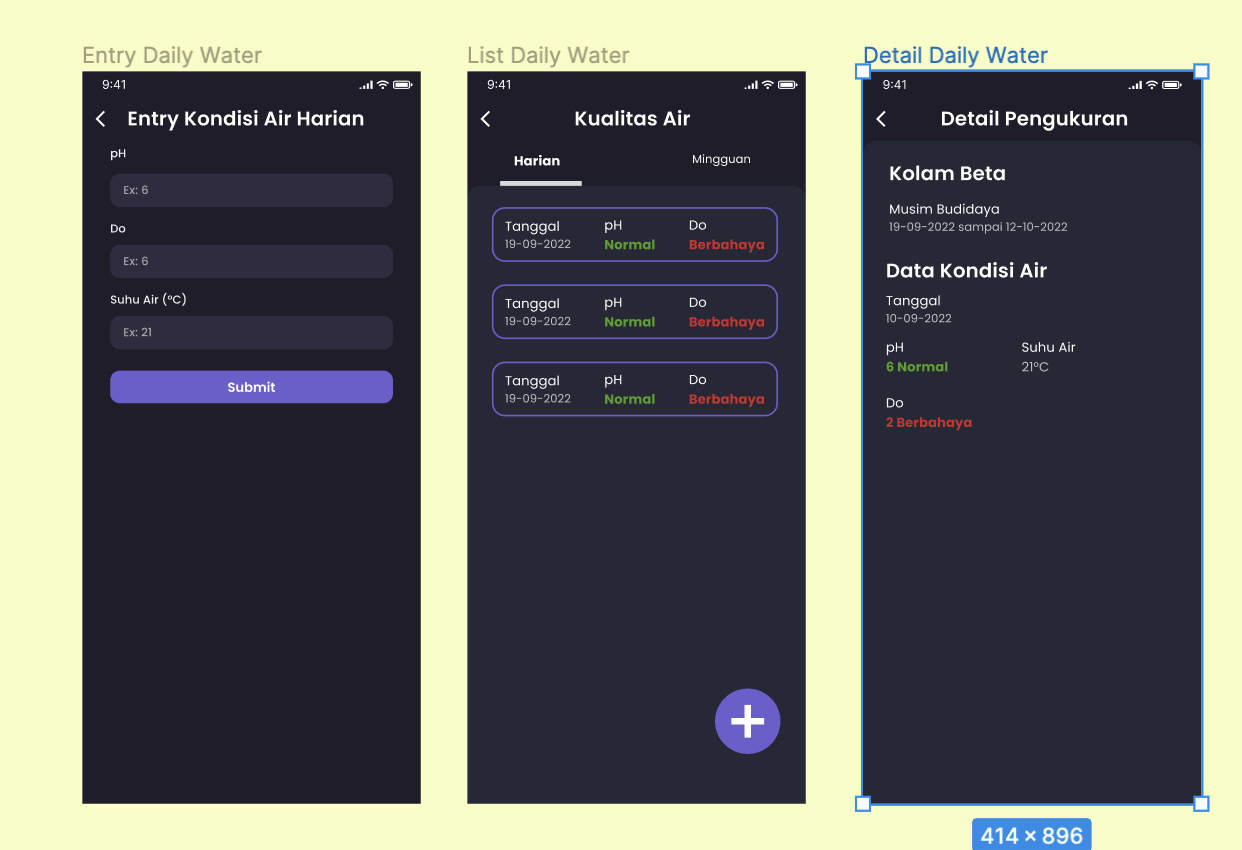
\includegraphics[keepaspectratio, width=6cm]{gambar/mockupairharian}
	\caption{\textit{Mock-up UI Fitur Pencatatan Kualitas Air Harian}}
	\label{gambar:mockupairharian}
	\end{figure}

	\item{\textit{Class Diagram}}
	
	Class Diagram menggambarkan kelas-kelas yang akan dipakai oleh sistem. Umumnya terdapat 3 kelas pada setiap module yaitu class model, controller, dan view. Pada sprint-8 penelitian kali ini penulis membuat 4 class yaitu model yang berwarna biru, view berwarna oranye, controller yang berwarna hijau, dan service yang berwarna kuning.
	 
	 \begin{figure}[H]
	 \centering
	 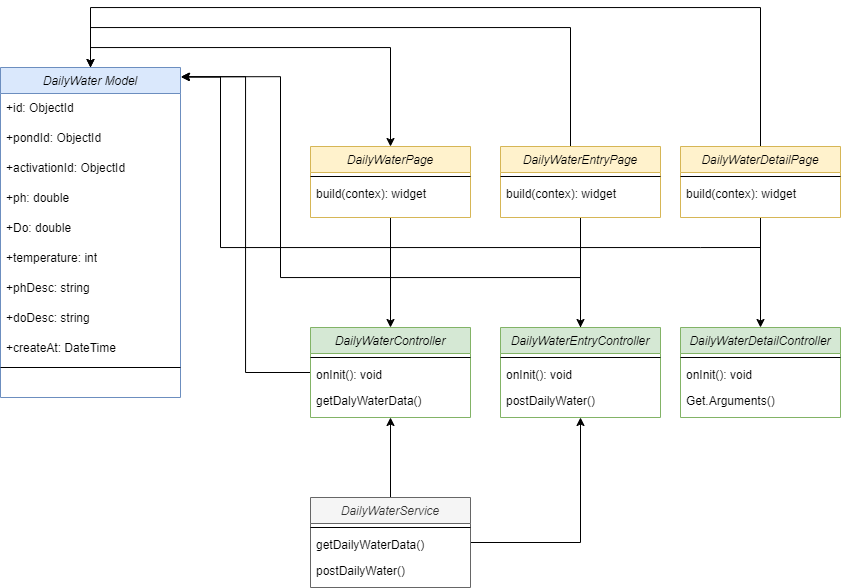
\includegraphics[keepaspectratio, width=6cm]{gambar/dailycd}
	 \caption{\textit{Class Diagram Fitur Sprint-8}}
	 \label{gambar:dailycd}
	 \end{figure}

	\item{\textit{Menerapkan Mockup-UI Fitur Pencatatan Kualitas Air Harian kedalam code flutter}}
	
	Setelah itu, akan dilakukan pengimplementasian \textit{mock-up UI} ke dalam aplikasi menggukan flutter. Pada lampiran 9 terdapat source code dari implementasi fitur pencatatan kualitas air harian yang dikelompokan berdasarkan halaman yang menghasilkan output halaman sebagai seperti dibawah ini.

	\begin{figure}[H]
		\centering
		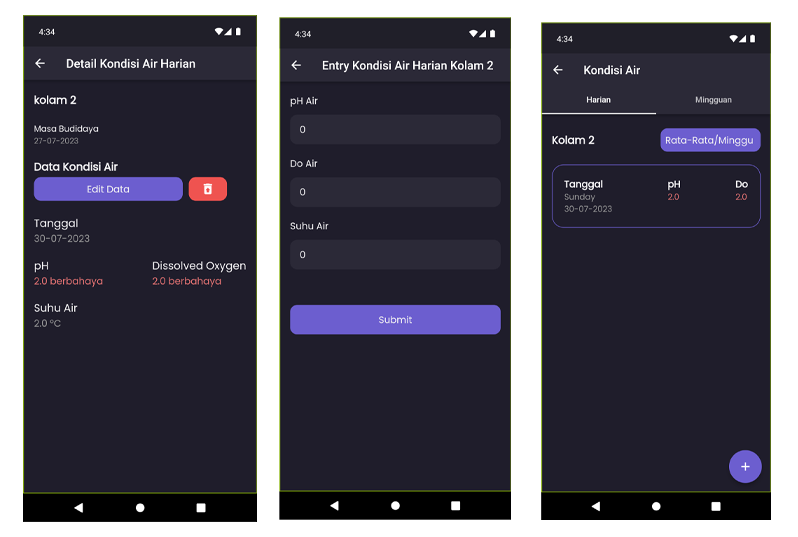
\includegraphics[keepaspectratio, width=8cm]{gambar/sssprint8}
		\caption{\textit{Output dari code pada sprint 8}}
		\label{gambar:sssprint8}
		\end{figure}

	\item{\textit{Mengitegrasikan fitur pencatatan kualitas air harian dengan webservice}}

	Sebelumnya, setiap data pada fitur masih berupa data dummy sehingga perlu diintegrasikan dengan webservice agar aplikasi dapat berjalan dengan data yang asli. Hal yang dilakukan dalam mengintegrasikan fitur pencatatan kualitas air harian dengan webservice terdapat pada lampiran 9.

  \item{Analisis \textit{User Experience}} 
 
  Pada halaman entry daily water quality, pembudidaya harus memasukan data yang diperlukan untuk melakukan daily water quality sesuai dengan kesepakatan saat meeting, seperti pH, Dissolved Oxygen, dan suhu. Selain itu terdapat juga list mengenai data daily water quality yang telah dimasukan yang berisi informasi yang berhubungan dengan daily water quality. Terdapat pula halaman detail daily water quality yang berisi informasi yang lebih detail terkait daily water quality yang telah dilakukan.

\item{Sprint 8 Review dan Sprint 9 Planning}

Sprint 8 diakhiri dengan melakukan weekly meeting pada hari selasa dengan agenda melakukan review dan testing terkait hasil sprint 8 dan melakukan planning untuk sprint 9 dengan rincian:
\begin{enumerate}
	\item{\textit{Review dan Testing hasil dari sprint 8}}

	Telah dilakukan review dan testing oleh penulis selaku developer dengan Scrum Master. Setelah dilakukan testing, Scrum Master menyimpulkan bahwa fitur pencatatan kualitas air harian telah berjalan dengan baik.

	\item{\textit{Sprint Planning untuk Sprint 9}}
	
	Planning untuk sprint 9 yakni membuat fitur pencatatan kualitas air mingguan pada aplikasi \textit{Assistive Aquaculture Breeding Management}.
\end{enumerate}
\end{enumerate}
%!TEX root = ./template-skripsi.tex

\subsection{\textit{Sprint 9}}

	\textit{Sprint-9} dilakukan sepekan pada tanggal 18 oktober 2022 sampai dengan 25 oktober 2022. \textit{Story} kesembilan pada \textit{product backlog} yaitu membuat fitur pencatatan kualitas air mingguan dipecah menjadi beberapa \textit{task} sebagai berikut.


 \begin{longtable}[c]{@{} |p{1cm}|p{4cm}|p{5cm}|p{3cm}| @{}}
 \caption{\textit{Sprint 9} \label{sprint9_table}}\\


 \hline
  \multirow{1}{=}{\centering{\textbf{No}}} & \multirow{1}{=}{\centering{\textbf{\textit{Story}}}} & \multirow{1}{=}{\centering{\textbf{\textit{Task}}}} & \multirow{1}{=}{\centering{\textbf{\textit{Status}}}}\\
 \endfirsthead

 \hline
  \multirow{1}{=}{\centering{\textbf{No}}} & \multirow{1}{=}{\centering{\textbf{\textit{Story}}}} & \multirow{1}{=}{\centering{\textbf{\textit{Task}}}} & \multirow{1}{=}{\centering{\textbf{\textit{Status}}}}\\
 \endhead

 \hline
 \endfoot

 \hline
 \endlastfoot

 \hline
 1 & Membuat fitur pencatatan kualitas air mingguan &  Membuat \textit{Mock-up UI} halaman list pencatatan kualitas air mingguan, entry kualitas air mingguan, detail kualitas air mingguan  &  selesai \\
 \hline
 2 & & Menerapkan \textit{Mock-up UI} halaman list pencatatan kualitas air mingguan, entry kualitas air mingguan, detail kualitas air mingguan ke Flutter & selesai\\
 \hline
 3 & & Mengintegrasikan halaman pencatatan kualitas air mingguan, entry kualitas air mingguan, detail kualitas air mingguan ke \textit{webservice} & selesai\\
 \hline
 \end{longtable}

Pada sprint kesembilan ini story yang di pilih untuk di uraikan pada sprint kali ini adalah membuat halaman pencatatan kualitas air mingguan, entry kualitas air mingguan, detail kualitas air mingguan. Tujuan dari \textit{sprint-9} ini adalah membuat fitur pencatatan kualitas air mingguan dan mengintegrasikan halaman tersebut dengan webservice yang sudah dibuat oleh penelitian Andri Rahmanto.

\begin{enumerate}[listparindent=2em]
	
	\item{\textit{Membuat Mock-up UI Fitur Pencatatan Kualitas air mingguan}}
	
	Pembuatan konten dan fitur yang terdapat pada \textit{mock-up UI} fitur pencatatan kualitas air mingguan dilakukan berdasarkan persetujuan product owner dan scrum master pada meeting sebelumnya. Mock-up UI dibuat menggunakan platform figma.
	
	\begin{figure}[H]
	\centering
	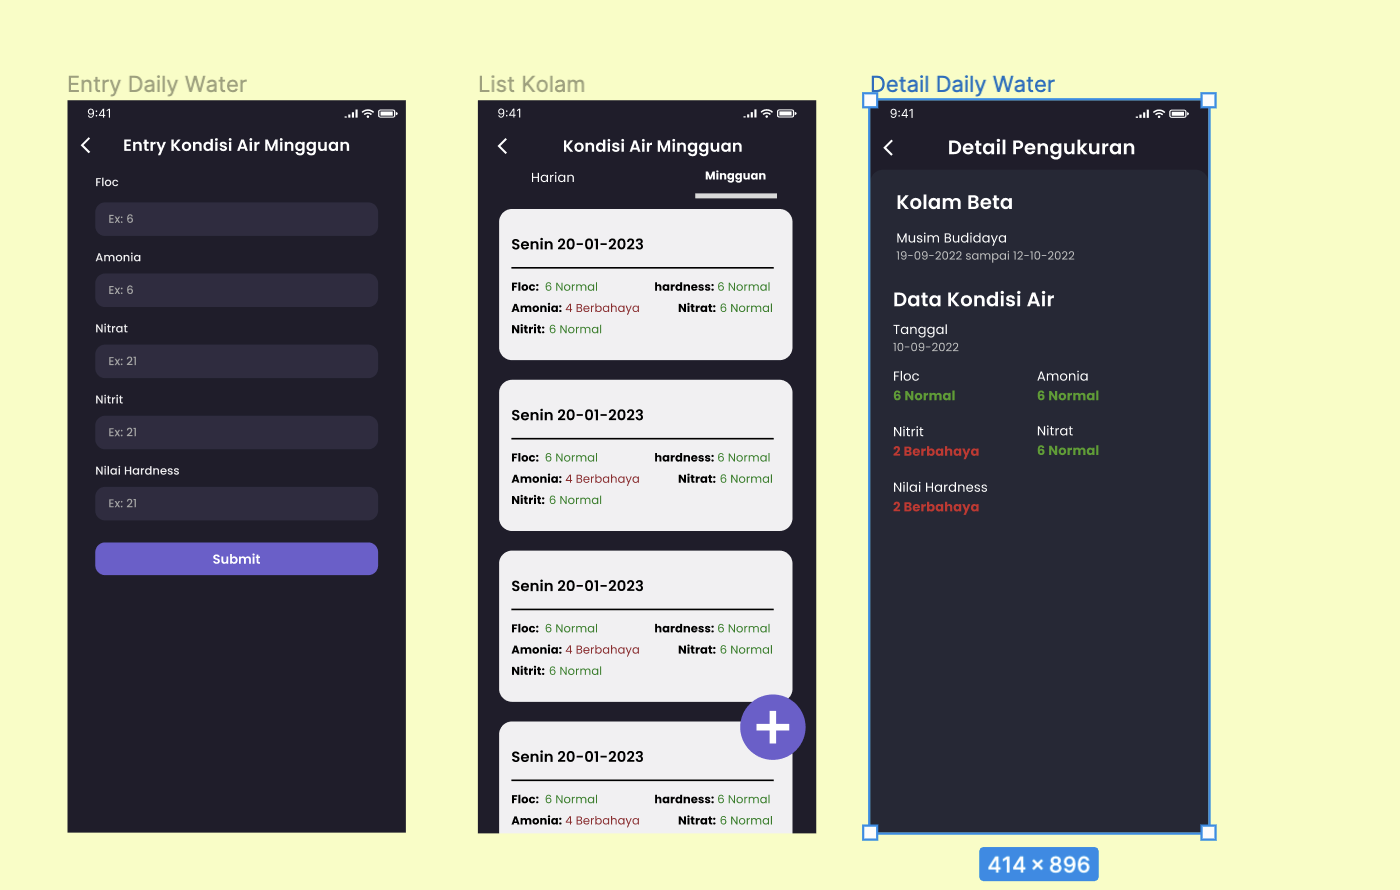
\includegraphics[keepaspectratio, width=6cm]{gambar/mockupairmingguan}
	\caption{\textit{Mock-up UI Fitur Pencatatan Kualitas air mingguan}}
	\label{gambar:mockupairmingguan}
	\end{figure}

	\item{\textit{Class Diagram}}
	
	Class Diagram menggambarkan kelas-kelas yang akan dipakai oleh sistem. Umumnya terdapat 3 kelas pada setiap module yaitu class model, controller, dan view. Pada sprint-9 penelitian kali ini penulis membuat 4 class yaitu model yang berwarna biru, view berwarna oranye, controller yang berwarna hijau, dan service yang berwarna kuning.
	 
	 \begin{figure}[H]
	 \centering
	 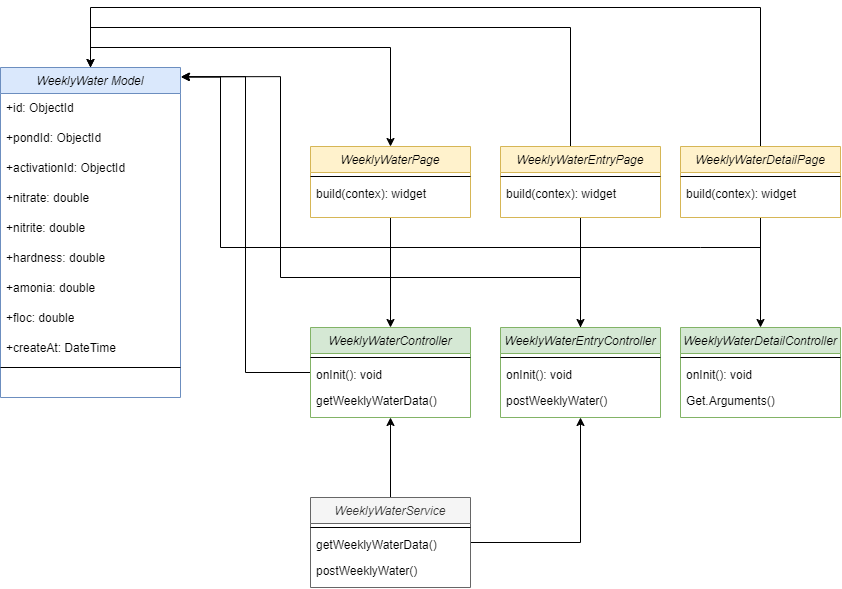
\includegraphics[keepaspectratio, width=6cm]{gambar/weeklycd}
	 \caption{\textit{Class Diagram Fitur Sprint-9}}
	 \label{gambar:weeklycd}
	 \end{figure}

	\item{\textit{Menerapkan Mockup-UI Fitur Pencatatan Kualitas air mingguan kedalam code flutter}}
	
	Setelah itu, akan dilakukan pengimplementasian \textit{mock-up UI} ke dalam aplikasi menggukan flutter. Pada lampiran 10 terdapat source code dari implementasi fitur pencatatan kualitas air mingguan yang dikelompokan berdasarkan halaman yang menghasilkan output halaman seperti dibawah ini

	\begin{figure}[H]
		\centering
		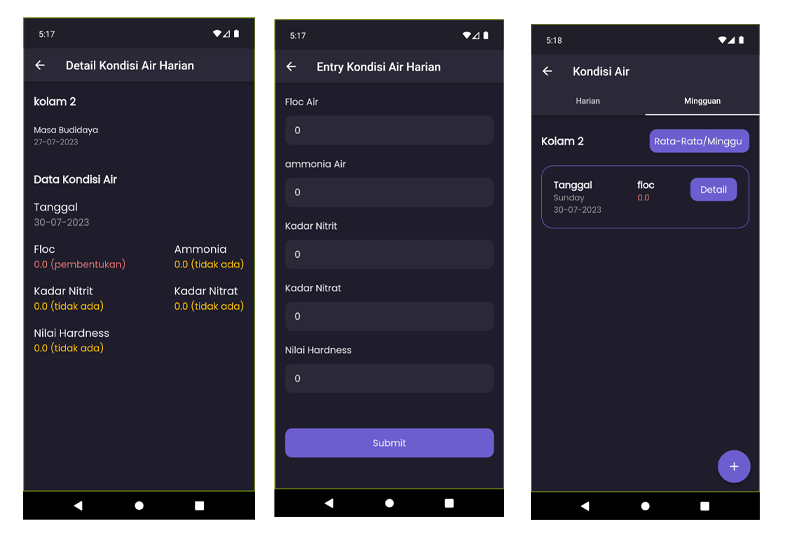
\includegraphics[keepaspectratio, width=8cm]{gambar/sssprint9}
		\caption{\textit{Output dari code pada sprint 9}}
		\label{gambar:sssprint9}
		\end{figure}

	\item{\textit{Mengitegrasikan fitur pencatatan kualitas air mingguan dengan webservice}}

	Sebelumnya, setiap data pada fitur masih berupa data dummy sehingga perlu diintegrasikan dengan webservice agar aplikasi dapat berjalan dengan data yang asli. Hal yang dilakukan dalam mengintegrasikan fitur pencatatan kualitas air mingguan dengan webservice terdapat pada lampiran 10.

  \item{Analisis \textit{User Experience}} 
 
  Pada halaman entry weekly water quality, pembudidaya harus memasukan data yang diperlukan untuk melakukan weekly water quality sesuai dengan kesepakatan saat meeting, seperti kadar nitrit, nitrat, amonia, dan nilai kekerasan air. Selain itu terdapat juga list mengenai data weekly water quality yang telah dimasukan yang berisi informasi yang berhubungan dengan weekly water quality. Terdapat pula halaman detail weekly water quality yang berisi informasi yang lebih detail terkait weekly water quality yang telah dilakukan.

\item{Sprint 9 Review dan Sprint 10 Planning}

Sprint 9 diakhiri dengan melakukan weekly meeting pada hari selasa dengan agenda melakukan review dan testing terkait hasil sprint 9 dan melakukan planning untuk sprint 10 dengan rincian:
\begin{enumerate}
	\item{\textit{Review dan Testing hasil dari sprint 9}}

	Telah dilakukan review dan testing oleh penulis selaku developer dengan Scrum Master. Setelah dilakukan testing, Scrum Master menyimpulkan bahwa fitur pencatatan kualitas air mingguan telah berjalan dengan baik.
	
  \begin{longtable}{| p{8cm} | c | c | l |}
    \caption{Unit testing Halaman Kualitas Air.\label{table:unit_testing_fitur_kualitas_air}}\\
    \hline
    \multirow{2}{*}{Skenario Pengujian} & \multicolumn{2}{l|}{Kesesuaian} & \multirow{2}{*}{Kesimpulan} \\ 
    \cline{2-3}
      & \multicolumn{1}{l|}{sesuai} & tidak sesuai & \\ 
    \hline
    \hline
    \endfirsthead
    \hline
    \multirow{2}{*}{Skenario Pengujian} & \multicolumn{2}{l|}{Kesesuaian} & \multirow{2}{*}{Kesimpulan} \\ 
    \cline{2-3}
      & \multicolumn{1}{l|}{sesuai} & tidak sesuai &  \\ 
    \hline
    \hline
    \endhead
    \hline
    \endfoot
    
    
    \hline\hline
    \endlastfoot
    Ketika memilih musim budidaya dan maka akan ditampilkan list pengontrolan kualitas air kolam & \Checkmark &  & Diterima \\ 
    \hline
    Ketika menekan list data pengontrolan kualitas air, maka akan ditamplikan detail pengontrolan kualitas air kolam & \Checkmark &  & Diterima \\ 
    \hline
    Saat ikon (+) ditekan maka akan menampilkan halaman entry pengontrolan kualitas air kolam & \Checkmark &  & Diterima \\ 
    \hline
    ketika mengisi form pengontrolan kualitas air kolam dengan data yang sesuai dan menekan submit, data pengontrolan kualitas air akan ditambahkan & \Checkmark &  & Diterima \\ 
    \hline
    \end{longtable}

	\item{\textit{Sprint Planning untuk Sprint 10}}
	
	Planning untuk sprint 10 yakni membuat fitur sortir kolam mingguan pada aplikasi \textit{Assistive Aquaculture Breeding Management}.
\end{enumerate}
\end{enumerate}
%!TEX root = ./template-skripsi.tex

\subsection{\textit{Sprint 10}}

	\textit{Sprint-10} dilakukan sepekan pada tanggal 25 oktober 2022 sampai dengan 1 november 2022. \textit{Story} kesepuluh pada \textit{product backlog} yaitu membuat fitur perpindahan antar kolam dipecah menjadi beberapa \textit{task} sebagai berikut.


 \begin{longtable}[c]{@{} |p{1cm}|p{4cm}|p{5cm}|p{3cm}| @{}}
 \caption{\textit{Sprint 10} \label{sprint10_table}}\\


 \hline
  \multirow{1}{=}{\centering{\textbf{No}}} & \multirow{1}{=}{\centering{\textbf{\textit{Story}}}} & \multirow{1}{=}{\centering{\textbf{\textit{Task}}}} & \multirow{1}{=}{\centering{\textbf{\textit{Status}}}}\\
 \endfirsthead

 \hline
  \multirow{1}{=}{\centering{\textbf{No}}} & \multirow{1}{=}{\centering{\textbf{\textit{Story}}}} & \multirow{1}{=}{\centering{\textbf{\textit{Task}}}} & \multirow{1}{=}{\centering{\textbf{\textit{Status}}}}\\
 \endhead

 \hline
 \endfoot

 \hline
 \endlastfoot

 \hline
 1 & Membuat fitur sortir kolam &  Membuat \textit{Mock-up UI} halaman list sortir, detail sortir, entry sortir &  selesai \\
 \hline
 2 & & Menerapkan \textit{Mock-up UI} halaman list sortir, detail sortir, entry sortir  ke Flutter & selesai\\
 \hline
 3 & & Mengintegrasikan halaman list soritr, entry soritr, detail soritr ke \textit{webservice} & selesai\\
 \hline
 \end{longtable}

Pada sprint kesepuluh ini story yang di pilih untuk di uraikan pada sprint kali ini adalah membuat fitur sortir. Tujuan dari \textit{sprint-10} ini adalah membuat fitur sortir ikan dan mengintegrasikan halaman tersebut dengan webservice yang sudah dibuat oleh penelitian Andri Rahmanto.

\begin{enumerate}[listparindent=2em]
	
	\item{\textit{Membuat Mock-up UI Fitur Sortir Kolam}}
	
	Pembuatan konten dan fitur yang terdapat pada \textit{mock-up UI} fitur sortir kolam dilakukan berdasarkan persetujuan product owner dan scrum master pada meeting sebelumnya. Mock-up UI dibuat menggunakan platform figma.
	
	\begin{figure}[H]
	\centering
	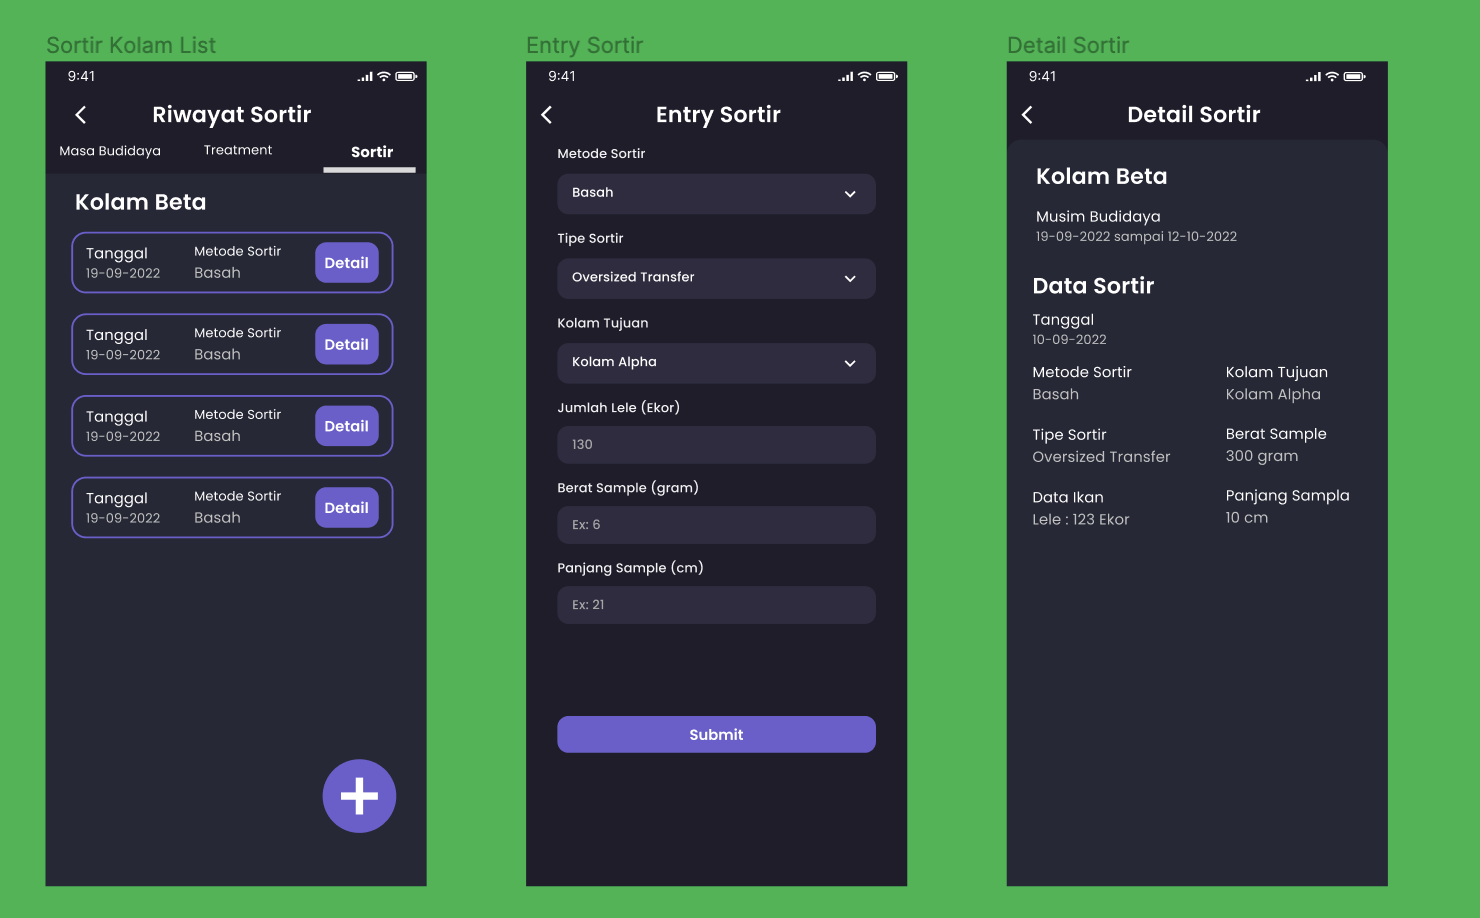
\includegraphics[keepaspectratio, width=10cm]{gambar/mockupsortir}
	\caption{\textit{Mock-up UI Fitur Sortir}}
	\label{gambar:mockupsortir}
	\end{figure}

	\item{\textit{Class Diagram}}
	
	Class Diagram menggambarkan kelas-kelas yang akan dipakai oleh sistem. Umumnya terdapat 3 kelas pada setiap module yaitu class model, controller, dan view. Pada sprint-10 penelitian kali ini penulis membuat 4 class yaitu model yang berwarna biru, view berwarna oranye, controller yang berwarna hijau, dan service yang berwarna kuning.
	 
	 \begin{figure}[H]
	 \centering
	 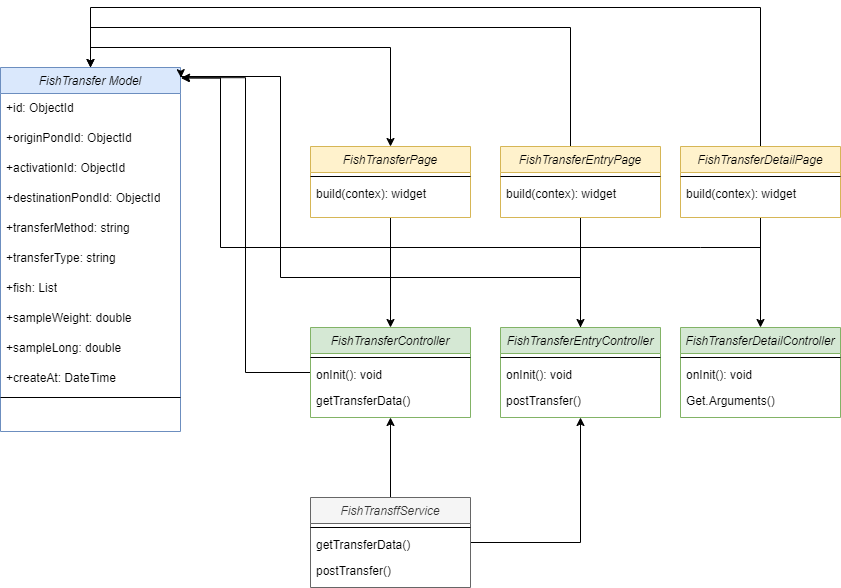
\includegraphics[keepaspectratio, width=6cm]{gambar/transfercd}
	 \caption{\textit{Class Diagram Fitur Sprint-10}}
	 \label{gambar:transfercd}
	 \end{figure}

	\item{\textit{Menerapkan Mockup-UI Fitur Sortir Kolam kedalam code flutter}}
	
	Setelah \textit{mock-up UI fitur Sortir kolam}, akan dilakukan pengimplementasian \textit{mock-up UI} ke dalam aplikasi menggukan flutter. Pada lampiran 11 terdapat source code dari implementasi fitur sortir yang dikelompokan berdasarkan halaman yang menghasilkan output halaman seperti dibawah ini.

	\begin{figure}[H]
		\centering
		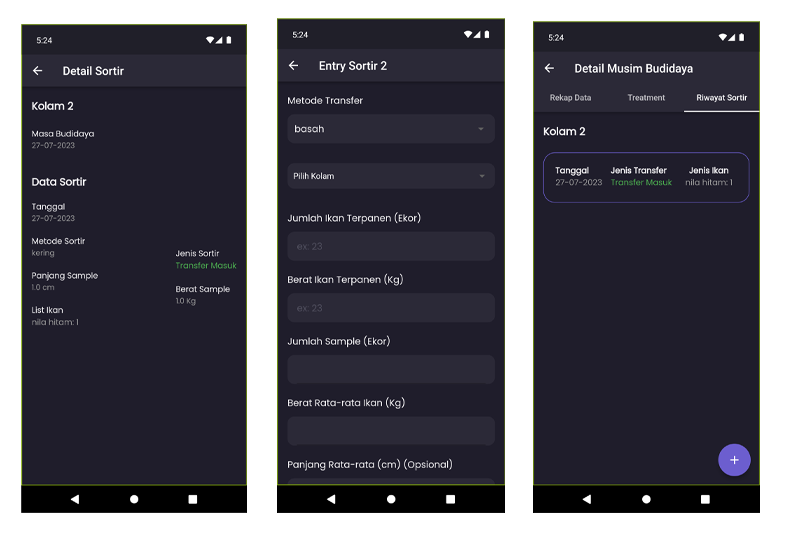
\includegraphics[keepaspectratio, width=8cm]{gambar/sssprint10}
		\caption{\textit{Output dari code pada sprint 10}}
		\label{gambar:sssprint10}
		\end{figure}

    \item{\textit{Mengitegrasikan fitur pencatatan kualitas air mingguan dengan webservice}}

	Sebelumnya, setiap data pada fitur masih berupa data dummy sehingga perlu diintegrasikan dengan webservice agar aplikasi dapat berjalan dengan data yang asli. Hal yang dilakukan dalam mengintegrasikan fitur sortir ikan dengan webservice terdapat pada lampiran 11.

  \item{Analisis \textit{User Experience}} 
 
  Pada halaman entry sortir kolam/transfer ikan, pembudidaya harus memasukan data yang diperlukan untuk melakukan sortir kolam/transfer ikan sesuai dengan kesepakatan saat meeting. Selain itu terdapat juga list mengenai data sortir kolam/transfer ikan yang telah dimasukan yang berisi informasi yang berhubungan dengan sortir kolam/transfer ikan. Terdapat pula halaman detail sortir kolam/transfer ikan yang berisi informasi yang lebih detail terkait sortir kolam/transfer ikan yang telah dilakukan.

\item{Sprint 10 Review dan Sprint 11 Planning}

Sprint 10 diakhiri dengan melakukan weekly meeting pada hari selasa dengan agenda melakukan review dan testing terkait hasil sprint 10 dan melakukan planning untuk sprint 11 dengan rincian:
\begin{enumerate}
	\item{\textit{Review dan Testing hasil dari sprint 10}}

	Telah dilakukan review dan testing oleh penulis selaku developer dengan Scrum Master. Setelah dilakukan testing, Scrum Master menyimpulkan bahwa fitur transfer/sortir ikam telah berjalan dengan baik.
	
  \begin{longtable}{| p{8cm} | c | c | l |}
    \caption{Unit testing Halaman Rekapitulasi Sortir.\label{table:unit_testing_rekapitulasi_sortir}}\\
    \hline
    \multirow{2}{*}{Skenario Pengujian} & \multicolumn{2}{l|}{Kesesuaian} & \multirow{2}{*}{Kesimpulan} \\ 
    \cline{2-3}
      & \multicolumn{1}{l|}{sesuai} & tidak sesuai & \\ 
    \hline
    \hline
    \endfirsthead
    \hline
    \multirow{2}{*}{Skenario Pengujian} & \multicolumn{2}{l|}{Kesesuaian} & \multirow{2}{*}{Kesimpulan} \\ 
    \cline{2-3}
      & \multicolumn{1}{l|}{sesuai} & tidak sesuai &  \\ 
    \hline
    \hline
    \endhead
    \hline
    \endfoot
    
    
    \hline\hline
    \endlastfoot
    Ketika menekan list data sortir, maka akan ditamplikan detail sortir & \Checkmark &  & Diterima \\ 
    \hline
    Saat ikon (+) ditekan maka akan menampilkan halaman entry sortir & \Checkmark &  & Diterima \\ 
    \hline
    ketika mengisi form sortir dengan data yang sesuai dan menekan submit, data sortir akan ditambahkan & \Checkmark &  & Diterima \\ 
    \hline
    \end{longtable}

	\item{\textit{Sprint Planning untuk Sprint 11}}
	
	Planning untuk sprint 11 yakni membuat fitur multi user pada aplikasi \textit{Assistive Aquaculture Breeding Management}.
\end{enumerate}
\end{enumerate}
%!TEX root = ./template-skripsi.tex

\subsection{\textit{Sprint 11}}

	\textit{Sprint-11} dilakukan sepekan pada tanggal 1 november 2022 sampai dengan 8 november 2022. \textit{Story} kesebelas pada \textit{product backlog} yaitu membuat fitur multiuser/login dan register dipecah menjadi beberapa \textit{task} sebagai berikut.


 \begin{longtable}[c]{@{} |p{1cm}|p{4cm}|p{5cm}|p{3cm}| @{}}
 \caption{\textit{Sprint 11} \label{sprint11_table}}\\


 \hline
  \multirow{1}{=}{\centering{\textbf{No}}} & \multirow{1}{=}{\centering{\textbf{\textit{Story}}}} & \multirow{1}{=}{\centering{\textbf{\textit{Task}}}} & \multirow{1}{=}{\centering{\textbf{\textit{Status}}}}\\
 \endfirsthead

 \hline
  \multirow{1}{=}{\centering{\textbf{No}}} & \multirow{1}{=}{\centering{\textbf{\textit{Story}}}} & \multirow{1}{=}{\centering{\textbf{\textit{Task}}}} & \multirow{1}{=}{\centering{\textbf{\textit{Status}}}}\\
 \endhead

 \hline
 \endfoot

 \hline
 \endlastfoot

 \hline
 1 & Membuat multiuser &  Membuat \textit{Mock-up UI} halaman login dan register &  selesai \\
 \hline
 2 & & Menerapkan \textit{Mock-up UI} halaman login dan register ke Flutter & selesai\\
 \hline
 3 & & Mengintegrasikan halaman login dan register ke \textit{webservice} & selesai\\
 \hline
 \end{longtable}

Pada sprint kesebelas ini story yang di pilih untuk di uraikan pada sprint kali ini adalah membuat login dan register. Tujuan dari \textit{sprint-11} ini adalah membuat multiuser dan mengintegrasikan halaman tersebut dengan webservice yang sudah dibuat oleh penelitian Andri Rahmanto.

\begin{enumerate}[listparindent=2em]
	
	\item{\textit{Membuat Mock-up UI Fitur multiuser}}
	
	Pembuatan konten dan fitur yang terdapat pada \textit{mock-up UI} fitur multiuser dilakukan berdasarkan persetujuan product owner dan scrum master pada meeting sebelumnya. Mock-up UI dibuat menggunakan platform figma.
	
	\begin{figure}[H]
	\centering
	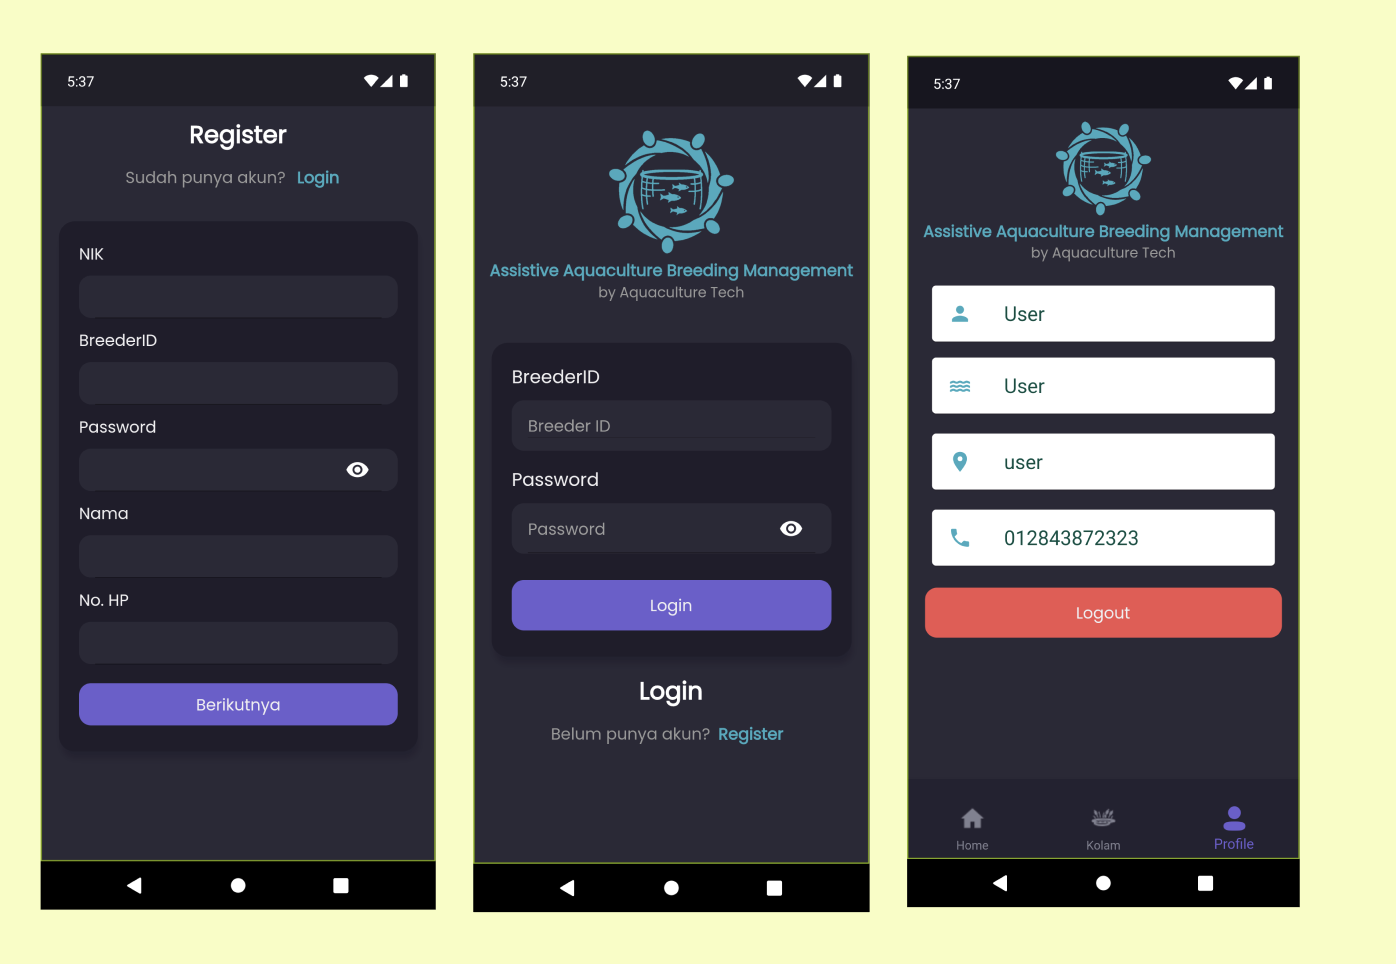
\includegraphics[keepaspectratio, width=6cm]{gambar/mockupmultiuser}
	\caption{\textit{Mock-up UI Fitur multiuser}}
	\label{gambar:mockupmultiuser}
	\end{figure}

	\item{\textit{Class Diagram}}
	
	Class Diagram menggambarkan kelas-kelas yang akan dipakai oleh sistem. Umumnya terdapat 3 kelas pada setiap module yaitu class model, controller, dan view. Pada sprint-11 penelitian kali ini penulis membuat 4 class yaitu model yang berwarna biru, view berwarna oranye, controller yang berwarna hijau, dan service yang berwarna kuning.
	 
	 \begin{figure}[H]
	 \centering
	 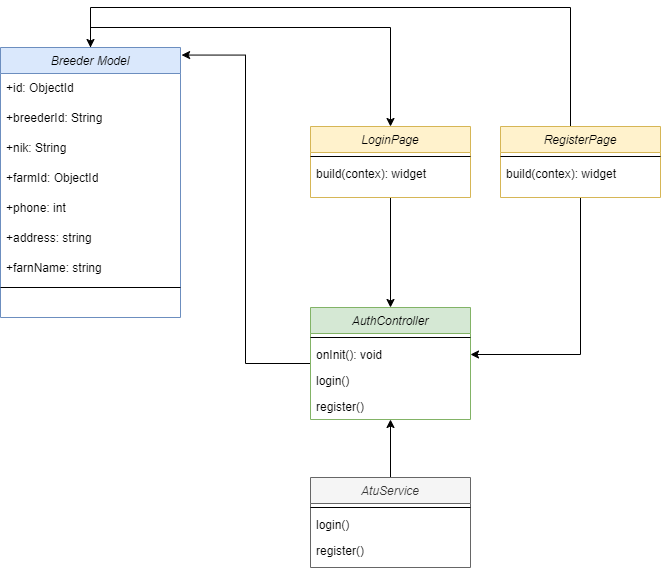
\includegraphics[keepaspectratio, width=6cm]{gambar/authcd}
	 \caption{\textit{Class Diagram Fitur Sprint-11}}
	 \label{gambar:authcd}
	 \end{figure}

	\item{\textit{Menerapkan Mockup-UI Fitur multiuser kedalam code flutter}}
	
	Setelah itu, akan dilakukan pengimplementasian \textit{mock-up UI} ke dalam aplikasi menggukan flutter. Pada lampiran 12 terdapat source code dari implementasi fitur multiuser yang dikelompokan berdasarkan halaman yang menghasilkan output halaman seperti pada gambar dibawah ini.

	\begin{figure}[H]
		\centering
		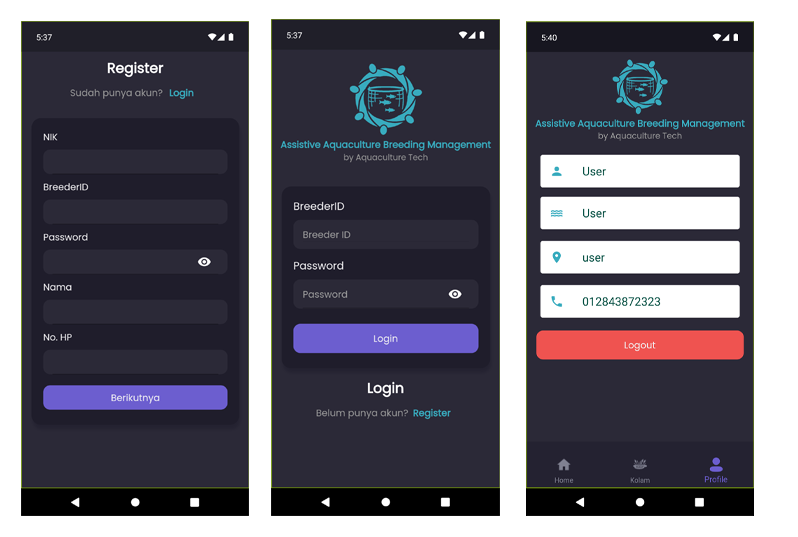
\includegraphics[keepaspectratio, width=8cm]{gambar/sssprint11}
		\caption{\textit{Output dari code pada sprint 11}}
		\label{gambar:sssprint11}
		\end{figure}

	\item{\textit{Mengitegrasikan fitur multiuser dengan webservice}}

    Hal yang dilakukan dalam mengintegrasikan fitur multiuser dengan webservice terpadat pada lampiran 12.

    \item{Analisis \textit{User Experience}} 
 
    Pada halaman register, pembudidaya harus memasukan data yang diperlukan untuk melakukan register sesuai dengan kesepakatan saat meeting. Setelah melakukan pendaftaran/register user dapat melakukan login dengan akun yang telah didaftarkan dengan menggunakan breeder ID dan password. Terdapat pula halaman profile yang berisi informasi yang terkait akun user/pembudidaya, dihalaman tersebut user dapat melakukan logout.
  

\item{Sprint 11 Review}

Sprint 11 diakhiri dengan melakukan weekly meeting pada hari selasa dengan agenda melakukan review dan testing terkait hasil sprint 11 dan melakukan planning untuk testing keseluruhan dengan rincian:
\begin{enumerate}
	\item{\textit{Review dan Testing hasil dari sprint 11}}

  Telah dilakukan review dan testing oleh penulis selaku developer dengan Scrum Master. Setelah dilakukan testing, Scrum Master menyimpulkan bahwa fitur multiuser telah berjalan dengan baik.

  \begin{longtable}{| p{8cm} | c | c | l |}
    \caption{Unit testing Halaman Awal.\label{table:unit_testing_fitur_awal}}\\
    \hline
    \multirow{2}{*}{Skenario Pengujian} & \multicolumn{2}{l|}{Kesesuaian} & \multirow{2}{*}{Kesimpulan} \\ 
    \cline{2-3}
      & \multicolumn{1}{l|}{sesuai} & tidak sesuai & \\ 
    \hline
    \hline
    \endfirsthead
    \hline
    \multirow{2}{*}{Skenario Pengujian} & \multicolumn{2}{l|}{Kesesuaian} & \multirow{2}{*}{Kesimpulan} \\ 
    \cline{2-3}
      & \multicolumn{1}{l|}{sesuai} & tidak sesuai &  \\ 
    \hline
    \hline
    \endhead
    \hline
    \endfoot
    
    
    \hline\hline
    \endlastfoot
    Saat aplikasi dibuka akan muncul splash screen yang menampilkan logo yang menandakan aplikasi sedang loading & \Checkmark &  & Diterima \\ 
    \hline
    Setelah loading selesai maka akan ditampikan halaman login & \Checkmark & & Diterima \\ 
    \hline
    \end{longtable}
    
    
    \begin{longtable}{| p{8cm} | c | c | l |}
    \caption{Unit testing Halaman Login.\label{table:unit_testing_fitur_login}}\\
    \hline
    \multirow{2}{*}{Skenario Pengujian} & \multicolumn{2}{l|}{Kesesuaian} & \multirow{2}{*}{Kesimpulan} \\ 
    \cline{2-3}
      & \multicolumn{1}{l|}{sesuai} & tidak sesuai & \\ 
    \hline
    \hline
    \endfirsthead
    \hline
    \multirow{2}{*}{Skenario Pengujian} & \multicolumn{2}{l|}{Kesesuaian} & \multirow{2}{*}{Kesimpulan} \\ 
    \cline{2-3}
      & \multicolumn{1}{l|}{sesuai} & tidak sesuai &  \\ 
    \hline
    \hline
    \endhead
    \hline
    \endfoot
    
    
    \hline\hline
    \endlastfoot
     Ketika mengisi form login dengan data yang sesuai kemudian menekan submit, maka akan masuk ke halaman dashboard & \Checkmark &  & Diterima \\ 
    \hline
     Ketika mengisi form login dengan data yang tidak sesuai kemudian menekan submit, maka akan menampilkan pesan kesalahan & \Checkmark & & Diterima \\ 
    \hline
    \end{longtable}
\end{enumerate}
\end{enumerate}

\section{Pengujian Sistem}
Pengujian sistem dilakukan menggunakan dua tipe yaitu Unit Testing dan User Acceptance Test (UAT). Pengujian dilaksanakan pada saat seluruh User Story pada Product Backlog telah diimplementasikan. Unit testing aplikasi dilakukan terhadap satu frontend developer, sedangkan pengujian User Acceptance Test dilakukan terhadap satu scrum master dan owner.

\subsection {Unit Testing}

Adapun hasil dari unit testing yang telah dilaksanakan kepada salah satu developer internal, pengujian tersebut dilakukan pada saat suatu fitur telah dinyatakan selesai yang dimana hasil unit testing tersebut telah dijelaskan pada masing masing sprint report sebelumnya. Kesimpulan dari unit testing yang telah dilakukan adalah fitur yang telah dibuat dapat berjalan dengan baik.

\subsection {User Acceptance Testing}

User Acceptance Test terhadap user dilaksanakan pada tanggal 22 April 2023 secara luring bertempat di kecamatan jasinga. Adapun hasil dari UAT yang telah dilaksanakan dapat dilihat pada tabel dibawah ini.

 \begin{longtable}[c]{@{} |p{1cm}|p{6.5cm}|p{1.1cm}|p{1.1cm}|p{1.1cm}|p{1.1cm}| @{}}
    \caption{\textit{User Acceptance Test} \label{user_testing}}\\
   
    \hline
    \multicolumn{6}{| c |}{\textbf{\textit{User Acceptance Test}}}\\
    \hline
     \multirow{2}{=}{\centering{\textbf{No}}} & \multirow{2}{=}{\centering{\textbf{\textit{Acceptance Requirements}}}} & \multicolumn{4}{| c |}{\textbf{Kesesuaian}}\\
    \cline{3-6}
      &  & \centering{\textbf{SS}} & \centering{\textbf{S}} & \centering{\textbf{TS}} & \centering{\textbf{STS}}
    \endfirsthead
   
    \hline
    \multicolumn{6}{| c |}{\textbf{\textit{User Acceptance Test}}}\\
    \hline
     \multirow{2}{=}{\centering{\textbf{No}}} & \multirow{2}{=}{\centering{\textbf{\textit{Acceptance Requirements}}}} & \multicolumn{4}{| c |}{\textbf{Kesesuaian}}\\
    \cline{3-6}
     &  & \centering{\textbf{SS}} & \centering{\textbf{S}} & \centering{\textbf{TS}} & \centering{\textbf{STS}}
    \endhead
   
    \hline
    \endfoot
   
    \hline
    \endlastfoot
   
    \hline
    1 & Fitur login sudah sesuai dengan kebutuhan pembudidaya & \Checkmark &  &  &\\
    \hline
    2 & Fitur dasboard sudah sesuai dengan kebutuhan pembudidaya & \Checkmark &  &  &\\
    \hline
    3 & Fitur registrasi, aktivasi dan deaktivasi sudah sesuai dengan kebutuhan pembudidaya &  &  & \Checkmark &\\
    \hline
    4 & Fitur pemberian dan rekapitulasi pakan sudah sesuai dengan kebutuhan pembudidaya &  & \Checkmark &  &\\
    \hline
    5 & Fitur grading berat ikan sudah sesuai dengan kebutuhan pembudidaya & \Checkmark &  &  &\\
    \hline
    6 & Fitur pencatatan kematian sudah sesuai dengan kebutuhan pembudidaya & \Checkmark &  &  &\\
    \hline
    7 & Fitur treatment kolam sudah sesuai dengan kebutuhan pembudidaya & \Checkmark &  &  &\\
    \hline
    8 & Fitur pencatatan kualitas air harian sudah sesuai dengan kebutuhan pembudidaya &  &  & \Checkmark &\\
    \hline
    9 & Fitur pencatatan kualitas air mingguan sudah sesuai dengan kebutuhan pembudidaya &  &  & \Checkmark &\\
    \hline
    10 & Fitur sortir ikan sudah sesuai dengan kebutuhan pembudidaya &  &  & \Checkmark &\\
    \hline
    \end{longtable}

Berdasarkan tabel diatas, terdapat empat fitur yang memerlukan revisi diantaranya:

\begin{enumerate}
	\item Pada fitur aktivasi kolam perlu ditambahkan input tipe aktivasi, yaitu pada saat melakukan aktivasi dapat memilih tipe aktivasinya dengan pilihan pembenihan dan pembesaran. 
	\item Pada fitur pencatatan kualitas air harian inputnya perlu diubah ke dalam bentuk desimal dikarenakan ukuran pH, Dissolved Oxygen. dan suhu dapat berupa desimal.
	\item Pada fitur pencatatan kualitas air mingguan inputnya perlu diubah ke dalam format desimal dikarenakan data yang di input dapat berupa desimal.
	\item Pada fitur sortir, terdapat perubahan flow dari fitur tersebut agar lebih sesuai dengan sortir ikan yang dilakukan oleh pembudidaya di lapangan.
\end{enumerate}

\subsection {Kesimpulan Pengujian}

Pengujian aplikasi dilaksanakan dengan dua metode yaitu unit testing dan User Acceptance Test (UAT). Berdasarkan uraian di atas, seluruh skenario pada unit testing terhadap satu internal developer berjalan dengan baik. Namun, berdasarkan hasil UAT terhadap pembudidaya terdapat beberapa masukan seperti fitur aktivasi kolam, pencatatan kualitas air, dan fitur sortir kolam.


%\subsection{\textit{Daily Scrum}}

%Pada akhir pekan di akhir setiap \textit{sprint}, akan diadakan \textit{voice call} untuk membahas perkembangan dan hambatan pada setiap \textit{sprint}.

% Baris ini digunakan untuk membantu dalam melakukan sitasi
% Karena diapit dengan comment, maka baris ini akan diabaikan
% oleh compiler LaTeX.
\begin{comment}
\bibliography{daftar-pustaka}
\end{comment}